% Options for packages loaded elsewhere
\PassOptionsToPackage{unicode}{hyperref}
\PassOptionsToPackage{hyphens}{url}
%
\documentclass[
  a4paper,
]{book}

\usepackage{amsmath,amssymb}
\usepackage{iftex}
\ifPDFTeX
  \usepackage[T1]{fontenc}
  \usepackage[utf8]{inputenc}
  \usepackage{textcomp} % provide euro and other symbols
\else % if luatex or xetex
  \usepackage{unicode-math}
  \defaultfontfeatures{Scale=MatchLowercase}
  \defaultfontfeatures[\rmfamily]{Ligatures=TeX,Scale=1}
\fi
\usepackage{lmodern}
\ifPDFTeX\else  
    % xetex/luatex font selection
\fi
% Use upquote if available, for straight quotes in verbatim environments
\IfFileExists{upquote.sty}{\usepackage{upquote}}{}
\IfFileExists{microtype.sty}{% use microtype if available
  \usepackage[]{microtype}
  \UseMicrotypeSet[protrusion]{basicmath} % disable protrusion for tt fonts
}{}
\makeatletter
\@ifundefined{KOMAClassName}{% if non-KOMA class
  \IfFileExists{parskip.sty}{%
    \usepackage{parskip}
  }{% else
    \setlength{\parindent}{0pt}
    \setlength{\parskip}{6pt plus 2pt minus 1pt}}
}{% if KOMA class
  \KOMAoptions{parskip=half}}
\makeatother
\usepackage{xcolor}
\usepackage[top=35mm,right=25mm,bottom=35mm,left=25mm,heightrounded]{geometry}
\setlength{\emergencystretch}{3em} % prevent overfull lines
\setcounter{secnumdepth}{-\maxdimen} % remove section numbering
% Make \paragraph and \subparagraph free-standing
\makeatletter
\ifx\paragraph\undefined\else
  \let\oldparagraph\paragraph
  \renewcommand{\paragraph}{
    \@ifstar
      \xxxParagraphStar
      \xxxParagraphNoStar
  }
  \newcommand{\xxxParagraphStar}[1]{\oldparagraph*{#1}\mbox{}}
  \newcommand{\xxxParagraphNoStar}[1]{\oldparagraph{#1}\mbox{}}
\fi
\ifx\subparagraph\undefined\else
  \let\oldsubparagraph\subparagraph
  \renewcommand{\subparagraph}{
    \@ifstar
      \xxxSubParagraphStar
      \xxxSubParagraphNoStar
  }
  \newcommand{\xxxSubParagraphStar}[1]{\oldsubparagraph*{#1}\mbox{}}
  \newcommand{\xxxSubParagraphNoStar}[1]{\oldsubparagraph{#1}\mbox{}}
\fi
\makeatother
\pagestyle{plain}


\providecommand{\tightlist}{%
  \setlength{\itemsep}{0pt}\setlength{\parskip}{0pt}}\usepackage{longtable,booktabs,array}
\usepackage{calc} % for calculating minipage widths
% Correct order of tables after \paragraph or \subparagraph
\usepackage{etoolbox}
\makeatletter
\patchcmd\longtable{\par}{\if@noskipsec\mbox{}\fi\par}{}{}
\makeatother
% Allow footnotes in longtable head/foot
\IfFileExists{footnotehyper.sty}{\usepackage{footnotehyper}}{\usepackage{footnote}}
\makesavenoteenv{longtable}
\usepackage{graphicx}
\makeatletter
\newsavebox\pandoc@box
\newcommand*\pandocbounded[1]{% scales image to fit in text height/width
  \sbox\pandoc@box{#1}%
  \Gscale@div\@tempa{\textheight}{\dimexpr\ht\pandoc@box+\dp\pandoc@box\relax}%
  \Gscale@div\@tempb{\linewidth}{\wd\pandoc@box}%
  \ifdim\@tempb\p@<\@tempa\p@\let\@tempa\@tempb\fi% select the smaller of both
  \ifdim\@tempa\p@<\p@\scalebox{\@tempa}{\usebox\pandoc@box}%
  \else\usebox{\pandoc@box}%
  \fi%
}
% Set default figure placement to htbp
\def\fps@figure{htbp}
\makeatother

\usepackage{hyphenat}
\usepackage{graphicx}
\usepackage{wallpaper} % for the background image on title page
\usepackage{geometry} % for margins
\usepackage{libertine}
\usepackage[most]{tcolorbox}
\usepackage{setspace}
\usepackage{parskip}
\usepackage{contour}
\usepackage{imakeidx}

\documentclass[openany]{book}


\makeindex[intoc=true]
\onehalfspacing % line spacing
\setlength{\parskip}{1.5em}
\setlength\parindent{0pt}
\makeatletter
\@ifpackageloaded{caption}{}{\usepackage{caption}}
\AtBeginDocument{%
\ifdefined\contentsname
  \renewcommand*\contentsname{Inhaltsverzeichnis}
\else
  \newcommand\contentsname{Inhaltsverzeichnis}
\fi
\ifdefined\listfigurename
  \renewcommand*\listfigurename{Abbildungsverzeichnis}
\else
  \newcommand\listfigurename{Abbildungsverzeichnis}
\fi
\ifdefined\listtablename
  \renewcommand*\listtablename{Tabellenverzeichnis}
\else
  \newcommand\listtablename{Tabellenverzeichnis}
\fi
\ifdefined\figurename
  \renewcommand*\figurename{Abbildung}
\else
  \newcommand\figurename{Abbildung}
\fi
\ifdefined\tablename
  \renewcommand*\tablename{Tabelle}
\else
  \newcommand\tablename{Tabelle}
\fi
}
\@ifpackageloaded{float}{}{\usepackage{float}}
\floatstyle{ruled}
\@ifundefined{c@chapter}{\newfloat{codelisting}{h}{lop}}{\newfloat{codelisting}{h}{lop}[chapter]}
\floatname{codelisting}{Listing}
\newcommand*\listoflistings{\listof{codelisting}{Listingverzeichnis}}
\makeatother
\makeatletter
\makeatother
\makeatletter
\@ifpackageloaded{caption}{}{\usepackage{caption}}
\@ifpackageloaded{subcaption}{}{\usepackage{subcaption}}
\makeatother
\makeatletter
\@ifpackageloaded{sidenotes}{}{\usepackage{sidenotes}}
\@ifpackageloaded{marginnote}{}{\usepackage{marginnote}}
\makeatother

\ifLuaTeX
\usepackage[bidi=basic]{babel}
\else
\usepackage[bidi=default]{babel}
\fi
\babelprovide[main,import]{ngerman}
% get rid of language-specific shorthands (see #6817):
\let\LanguageShortHands\languageshorthands
\def\languageshorthands#1{}
\ifLuaTeX
  \usepackage[german]{selnolig} % disable illegal ligatures
\fi
\usepackage{bookmark}

\IfFileExists{xurl.sty}{\usepackage{xurl}}{} % add URL line breaks if available
\urlstyle{same} % disable monospaced font for URLs
\hypersetup{
  pdftitle={Gallery Grid},
  pdflang={de},
  hidelinks,
  pdfcreator={LaTeX via pandoc}}


\title{Gallery Grid}
\author{}
\date{}

\begin{document}
  \begin{frontmatter}
  \begin{titlepage}
  %  SOURCE: https://github.com/nmfs-opensci/quarto_titlepages_v1/tree/main

  % This is a combination of Pandoc templating and LaTeX
  % Pandoc templating https://pandoc.org/MANUAL.html#templates

  \tcbset{ % parameters for text background 
      frame code={},
      left=0pt, % margins
      right=0pt,
      top=0pt,
      bottom=0pt,
      colback=gray!10!black, % box color
      width=\dimexpr\textwidth\relax, 
      boxsep=15pt, % spacing between boxes
      arc=0pt, % no rounded edges
      opacityback=0.35, % translucent-ish background
      fontupper=\color{white}, % fontcolor
      fontlower=\color{white}
      }



  % background image
    \ThisLRCornerWallPaper{1.1}{images/fmd10024322a.jpg}  

  \begin{tcolorbox}


  \centering

  % Title and subtitle
  {\Huge\bfseries\nohyphens{Gallery Grid}}\\[1\baselineskip]

  \end{tcolorbox}

  \bigbreak

  % Authors
  \begin{tcolorbox}

    

  %%%%%% Affiliations
  \vspace{2\baselineskip} 

  \hangindent=1em
  \hangafter=1


  %%%%%% Correspondence
  \vspace{1\baselineskip} 


  \end{tcolorbox}


  %use \vfill instead to get the space to fill flexibly	
  %\vspace{0.25\textheight} % Whitespace between the title block and the publisher

  \vfill

  % Whitespace between the title block and the tagline
  \vspace{1\baselineskip} 

  \begin{tcolorbox}
  \centering

  %%%%%% Tagline at bottom
  {
    TIB\\
    Open Science Lab
  }
  \end{tcolorbox}
  \end{titlepage}
  \end{frontmatter}


\tableofcontents
{\let\newpage\relax}

\mainmatter
\begin{figure*}

\begin{figure}[H]    
  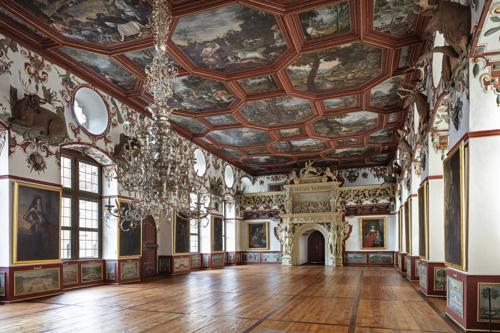
\includegraphics[height=10cm]{https://previous.bildindex.de/bilder/fmd10005862a.jpg}
  \caption{Knight's Hall + Room 72 - to the west}
  \label{fig:{https://previous.bildindex.de/bilder/fmd10005862a.jpg}}
\end{figure}

\clearpage

\begin{figure}[H]    
  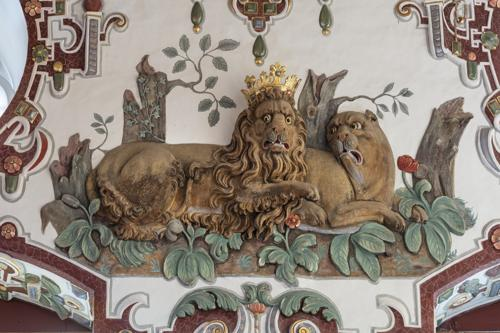
\includegraphics[height=10cm]{https://previous.bildindex.de/bilder/fmd10005864a.jpg}
  \caption{Lion couple – general view}
  \label{fig:{https://previous.bildindex.de/bilder/fmd10005864a.jpg}}
\end{figure}

\clearpage

\begin{figure}[H]    
  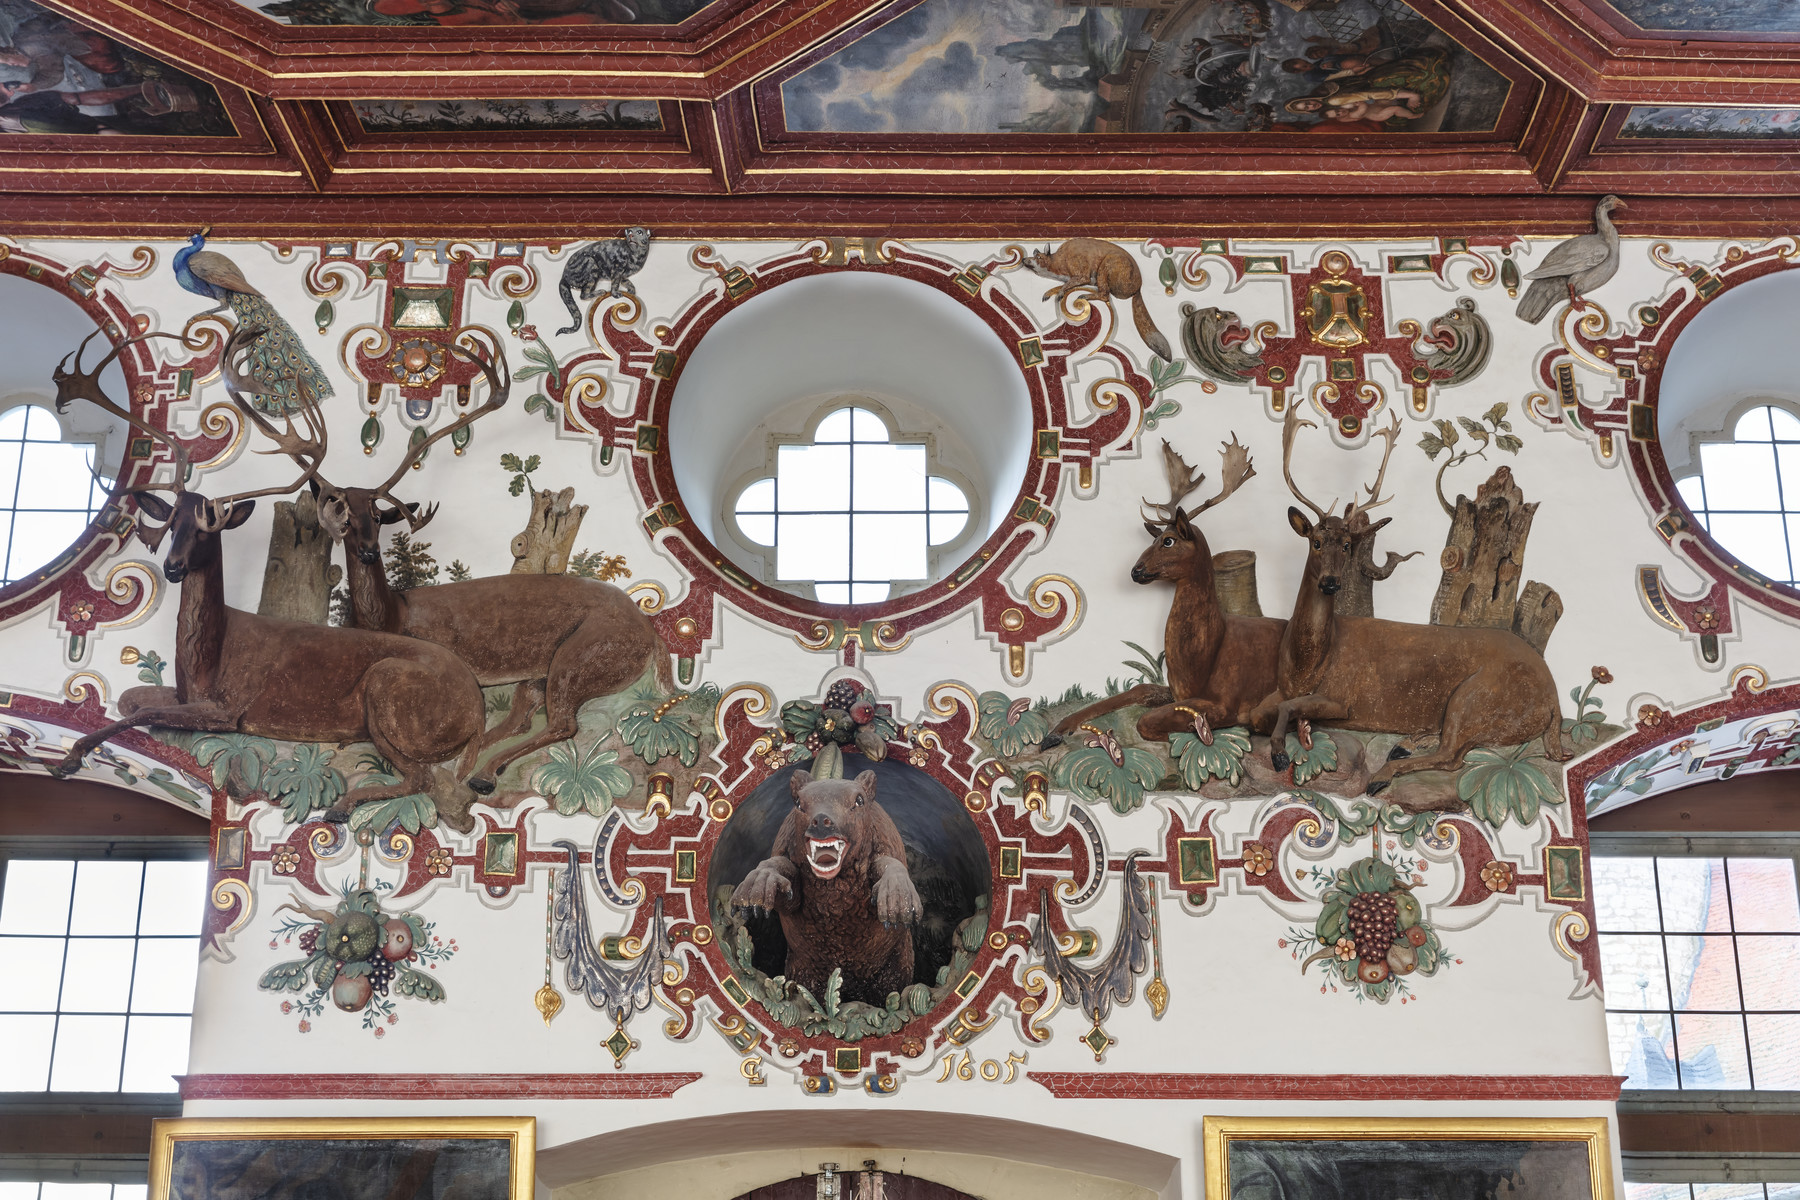
\includegraphics[height=10cm]{https://previous.bildindex.de/bilder/fmd10005865a.jpg}
  \caption{Bear – general view}
  \label{fig:{https://previous.bildindex.de/bilder/fmd10005865a.jpg}}
\end{figure}

\clearpage

\begin{figure}[H]    
  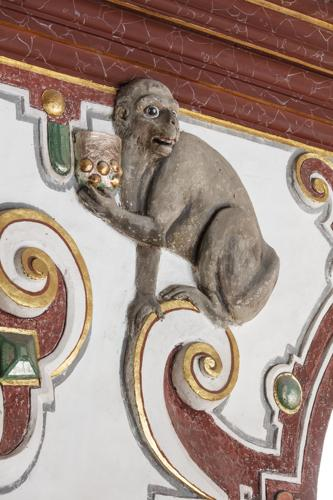
\includegraphics[height=10cm]{https://previous.bildindex.de/bilder/fmd10005867a.jpg}
  \caption{Monkey – general view}
  \label{fig:{https://previous.bildindex.de/bilder/fmd10005867a.jpg}}
\end{figure}

\clearpage

\begin{figure}[H]    
  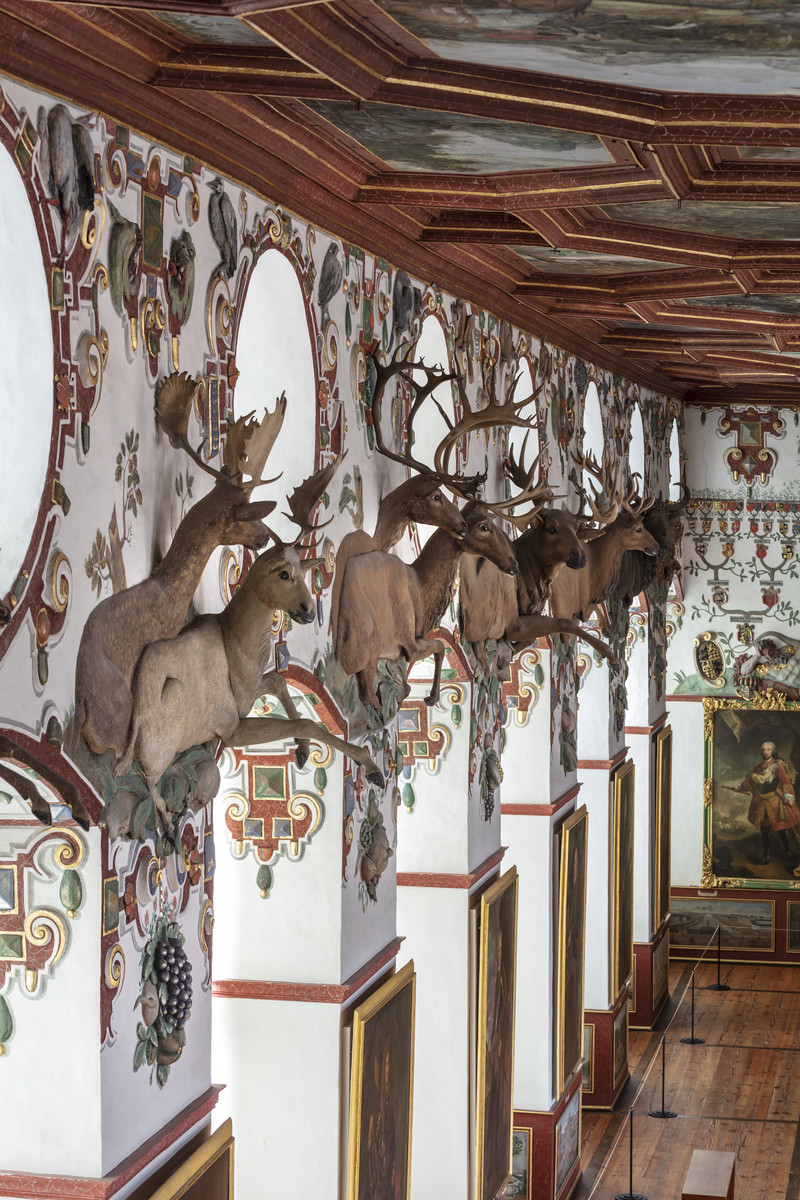
\includegraphics[height=10cm]{https://previous.bildindex.de/bilder/fmd10005866a.jpg}
  \caption{Deer pairs – general view}
  \label{fig:{https://previous.bildindex.de/bilder/fmd10005866a.jpg}}
\end{figure}

\clearpage

\begin{figure}[H]    
  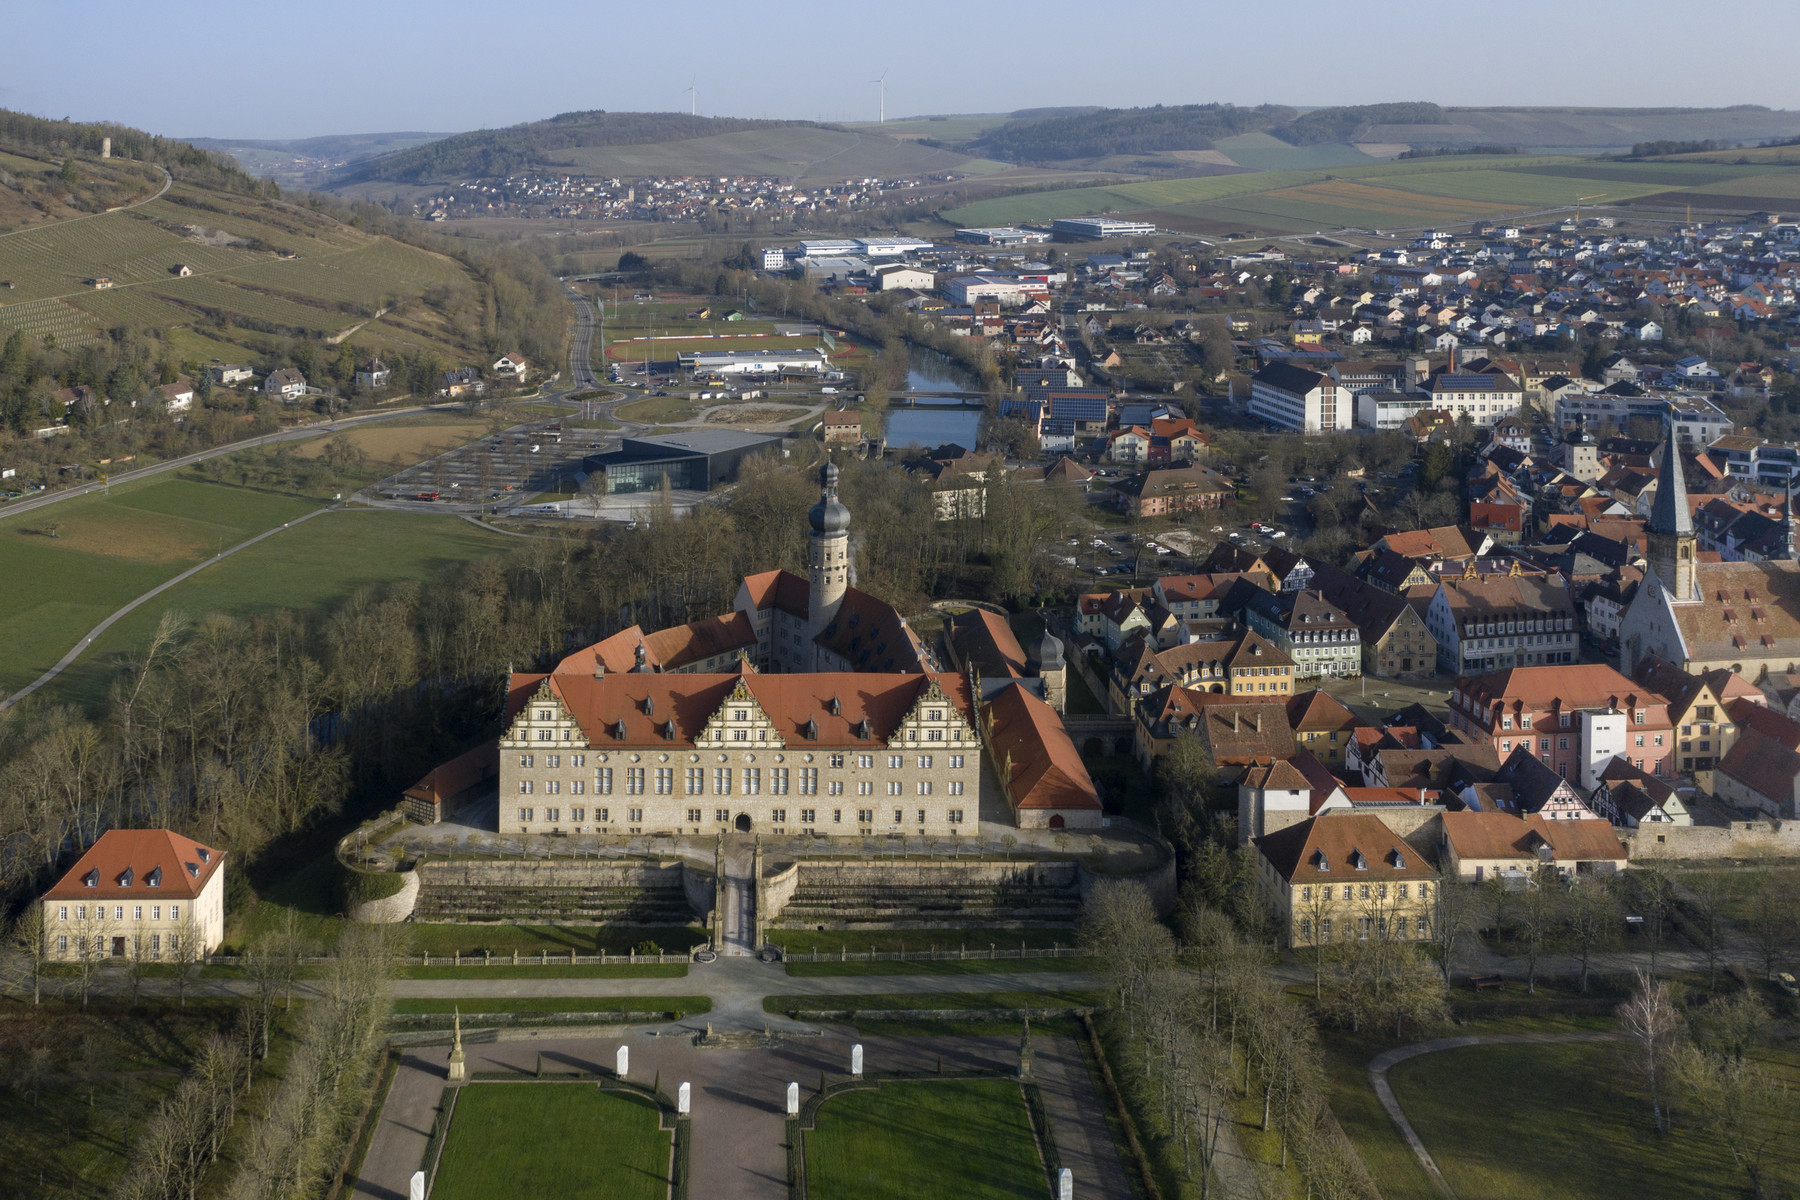
\includegraphics[height=10cm]{https://previous.bildindex.de/bilder/fmd10024321a.jpg}
  \caption{Hall building - garden side of the palace from the south}
  \label{fig:{https://previous.bildindex.de/bilder/fmd10024321a.jpg}}
\end{figure}

\clearpage

\begin{figure}[H]    
  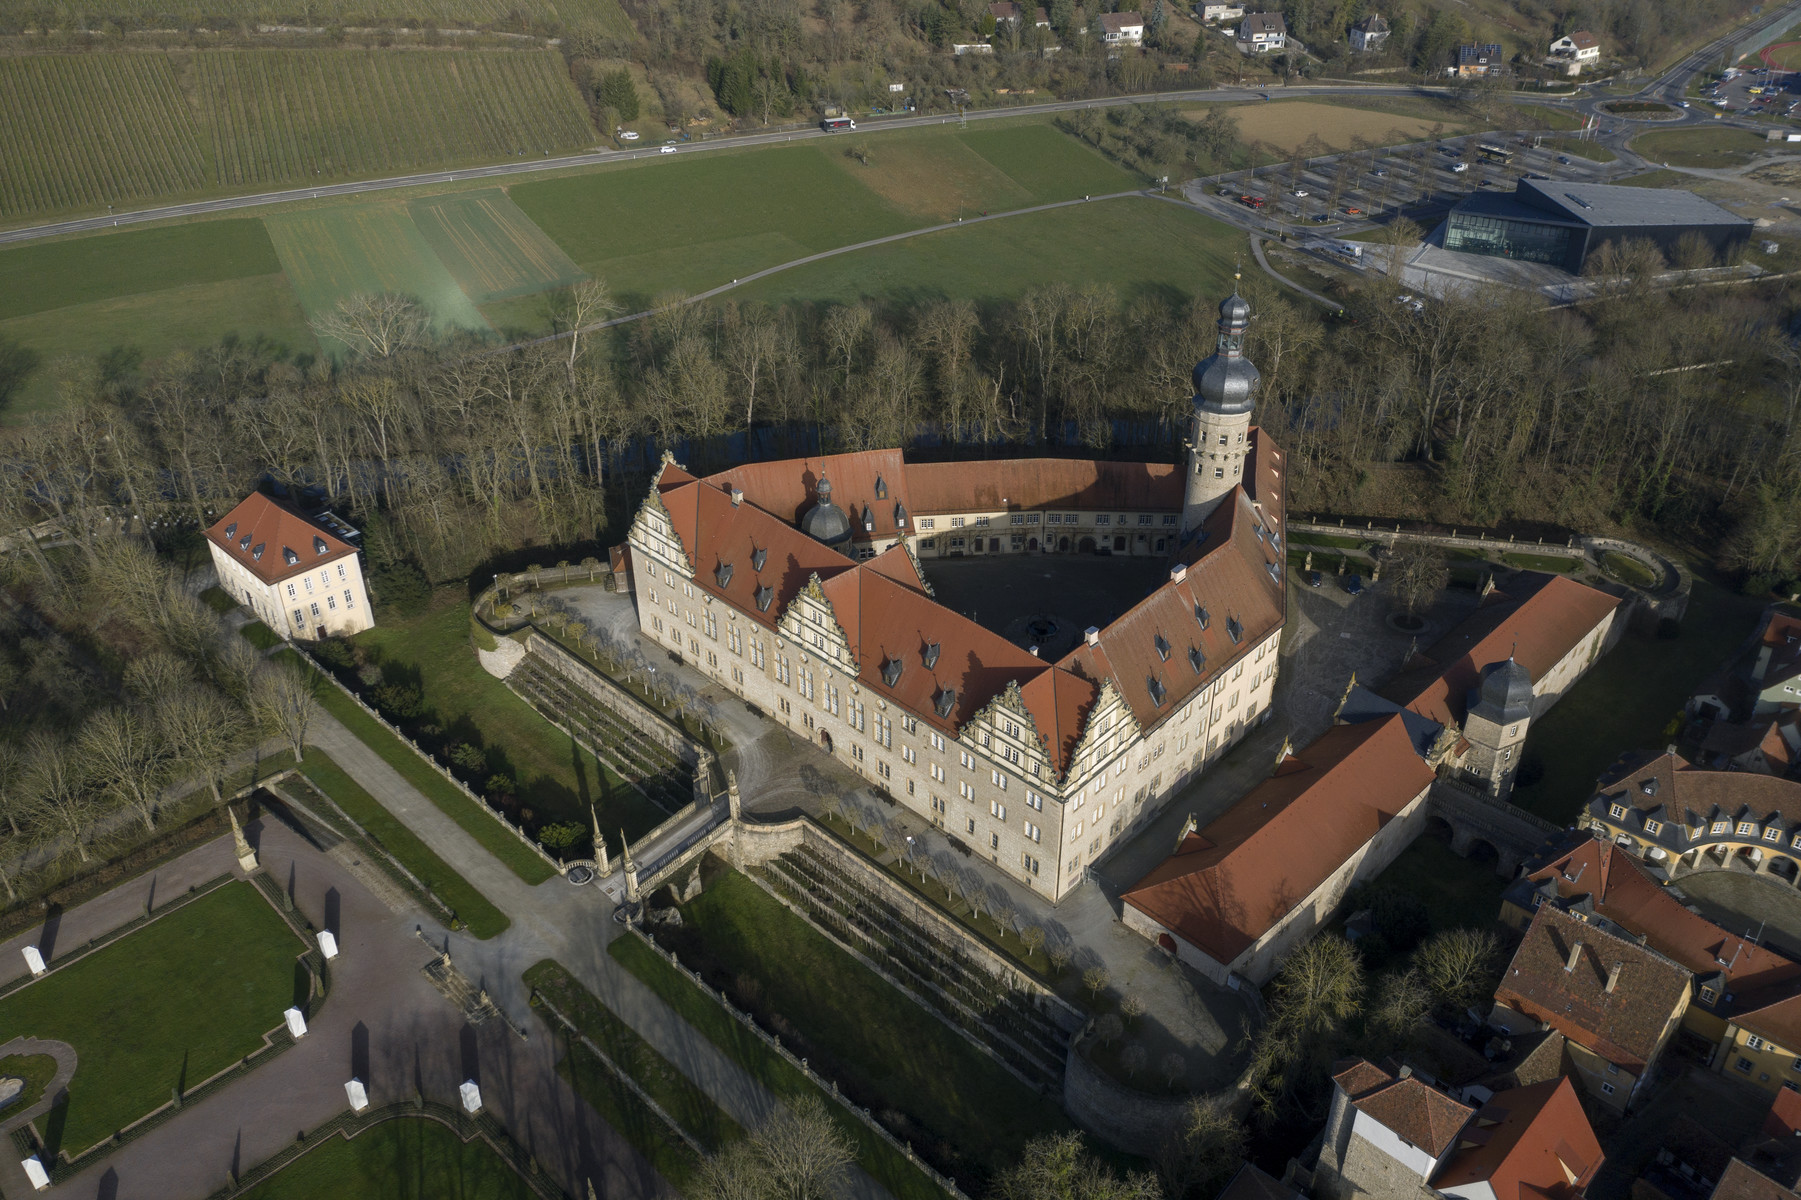
\includegraphics[height=10cm]{https://previous.bildindex.de/bilder/fmd10024322a.jpg}
  \caption{Saalbau - from the south-east}
  \label{fig:{https://previous.bildindex.de/bilder/fmd10024322a.jpg}}
\end{figure}

\clearpage

\begin{figure}[H]    
  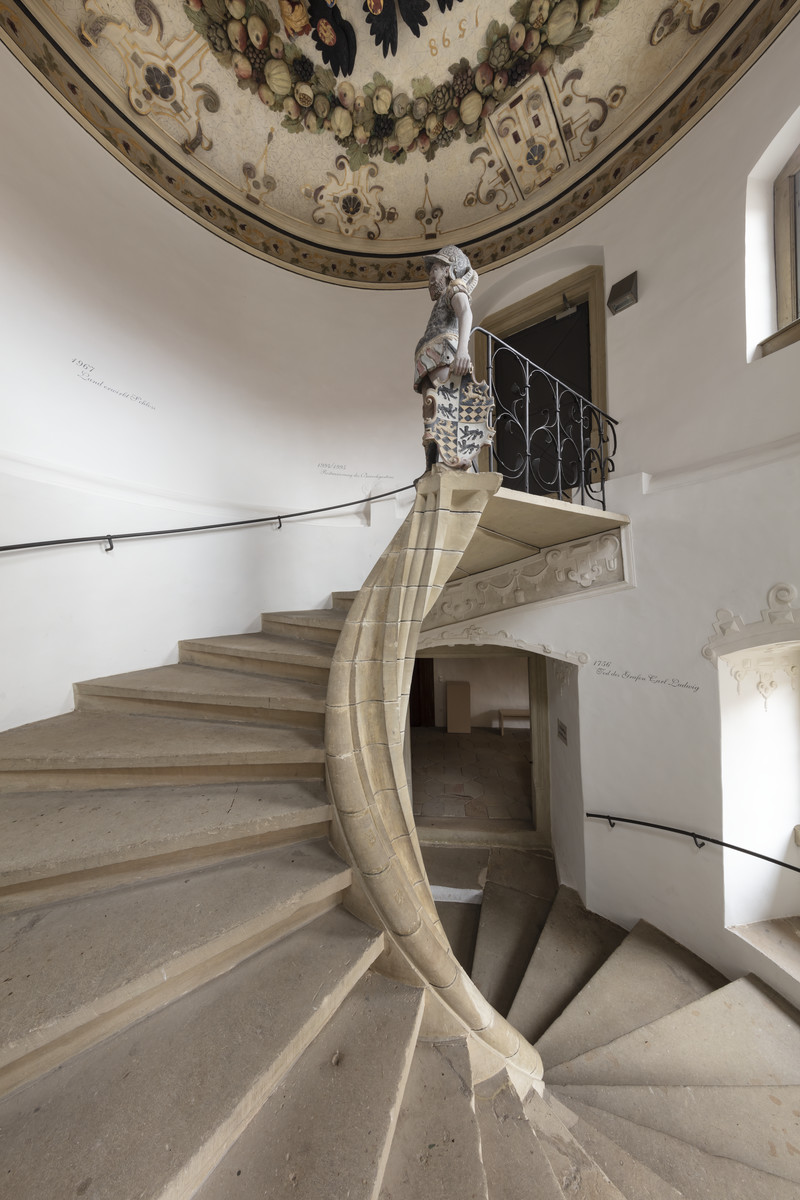
\includegraphics[height=10cm]{https://previous.bildindex.de/bilder/fmd10005853a.jpg}
  \caption{Development space sequences}
  \label{fig:{https://previous.bildindex.de/bilder/fmd10005853a.jpg}}
\end{figure}

\clearpage

\begin{figure}[H]    
  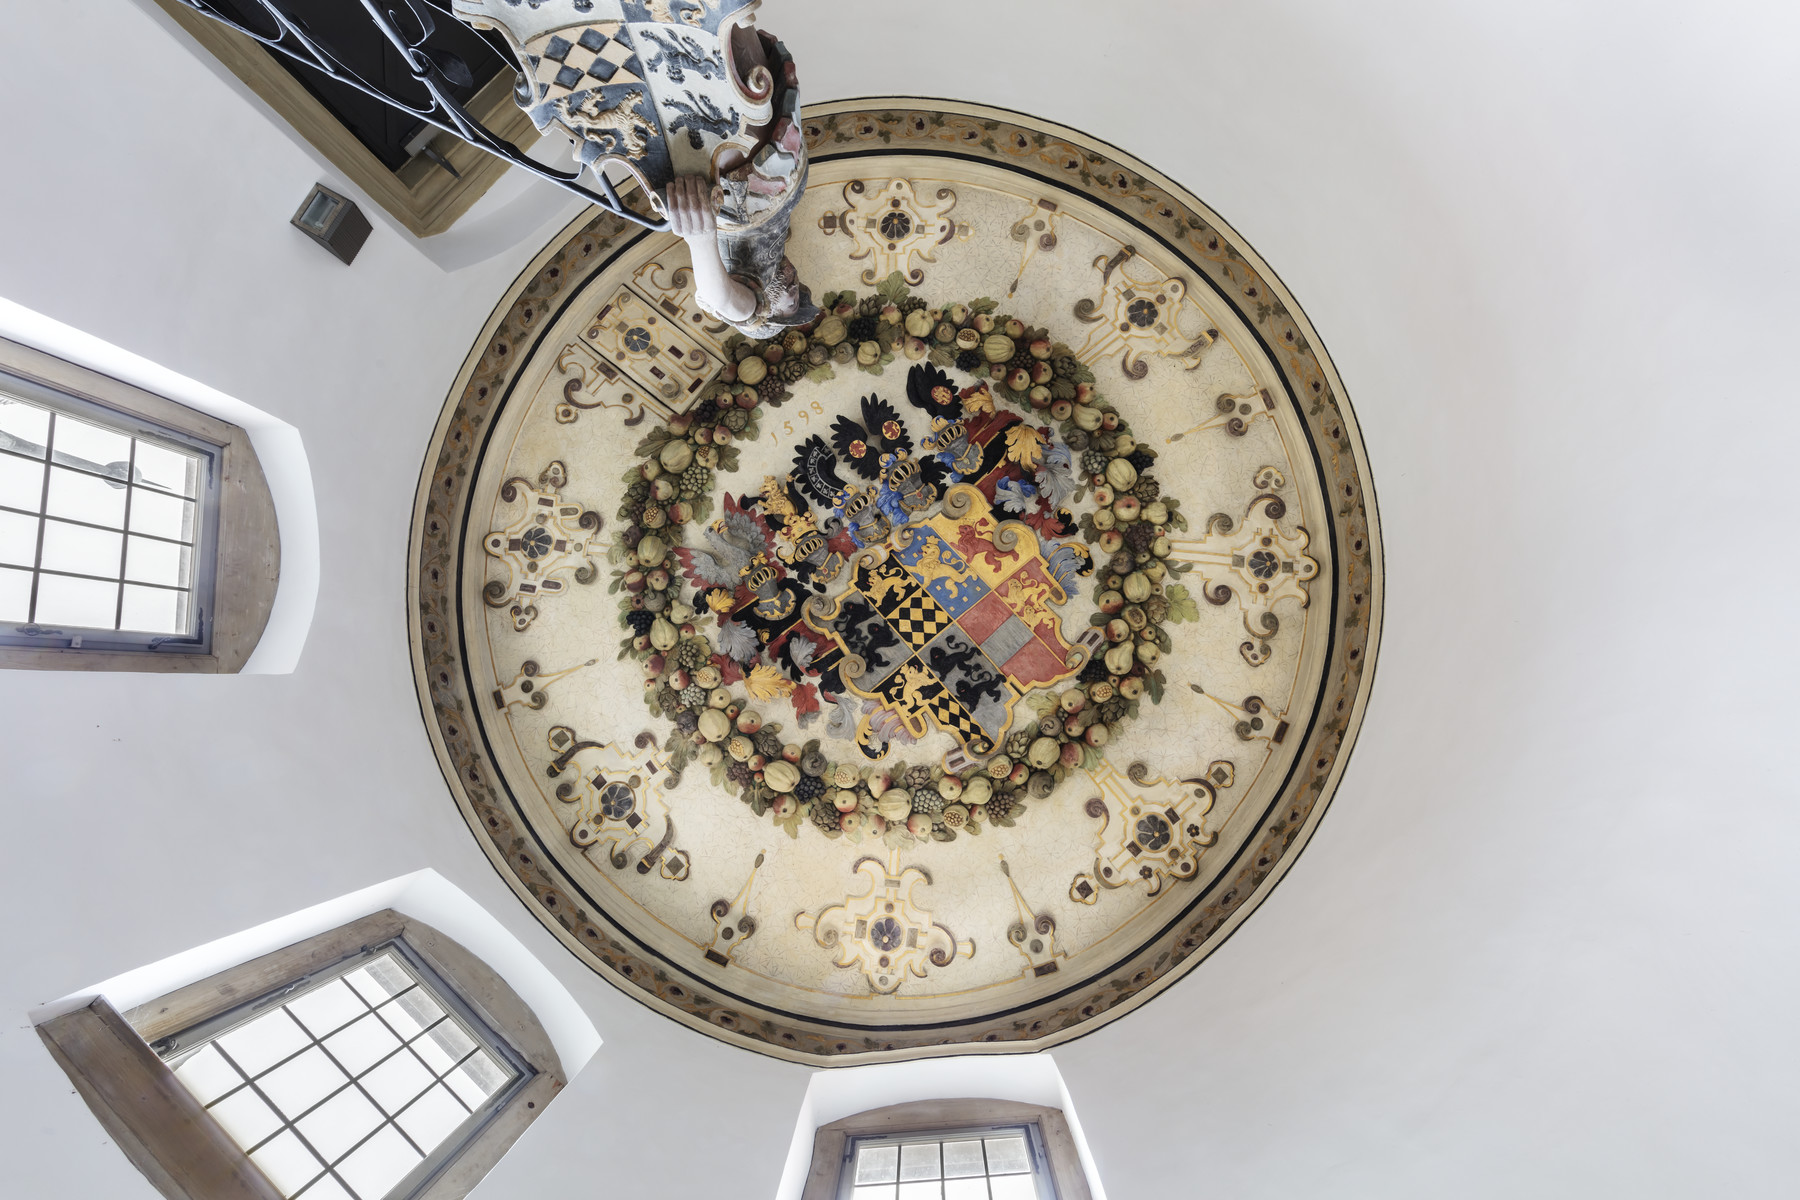
\includegraphics[height=10cm]{https://previous.bildindex.de/bilder/fmd10005854a.jpg}
  \caption{Ceiling decoration on stairwell}
  \label{fig:{https://previous.bildindex.de/bilder/fmd10005854a.jpg}}
\end{figure}

\clearpage

\begin{figure}[H]    
  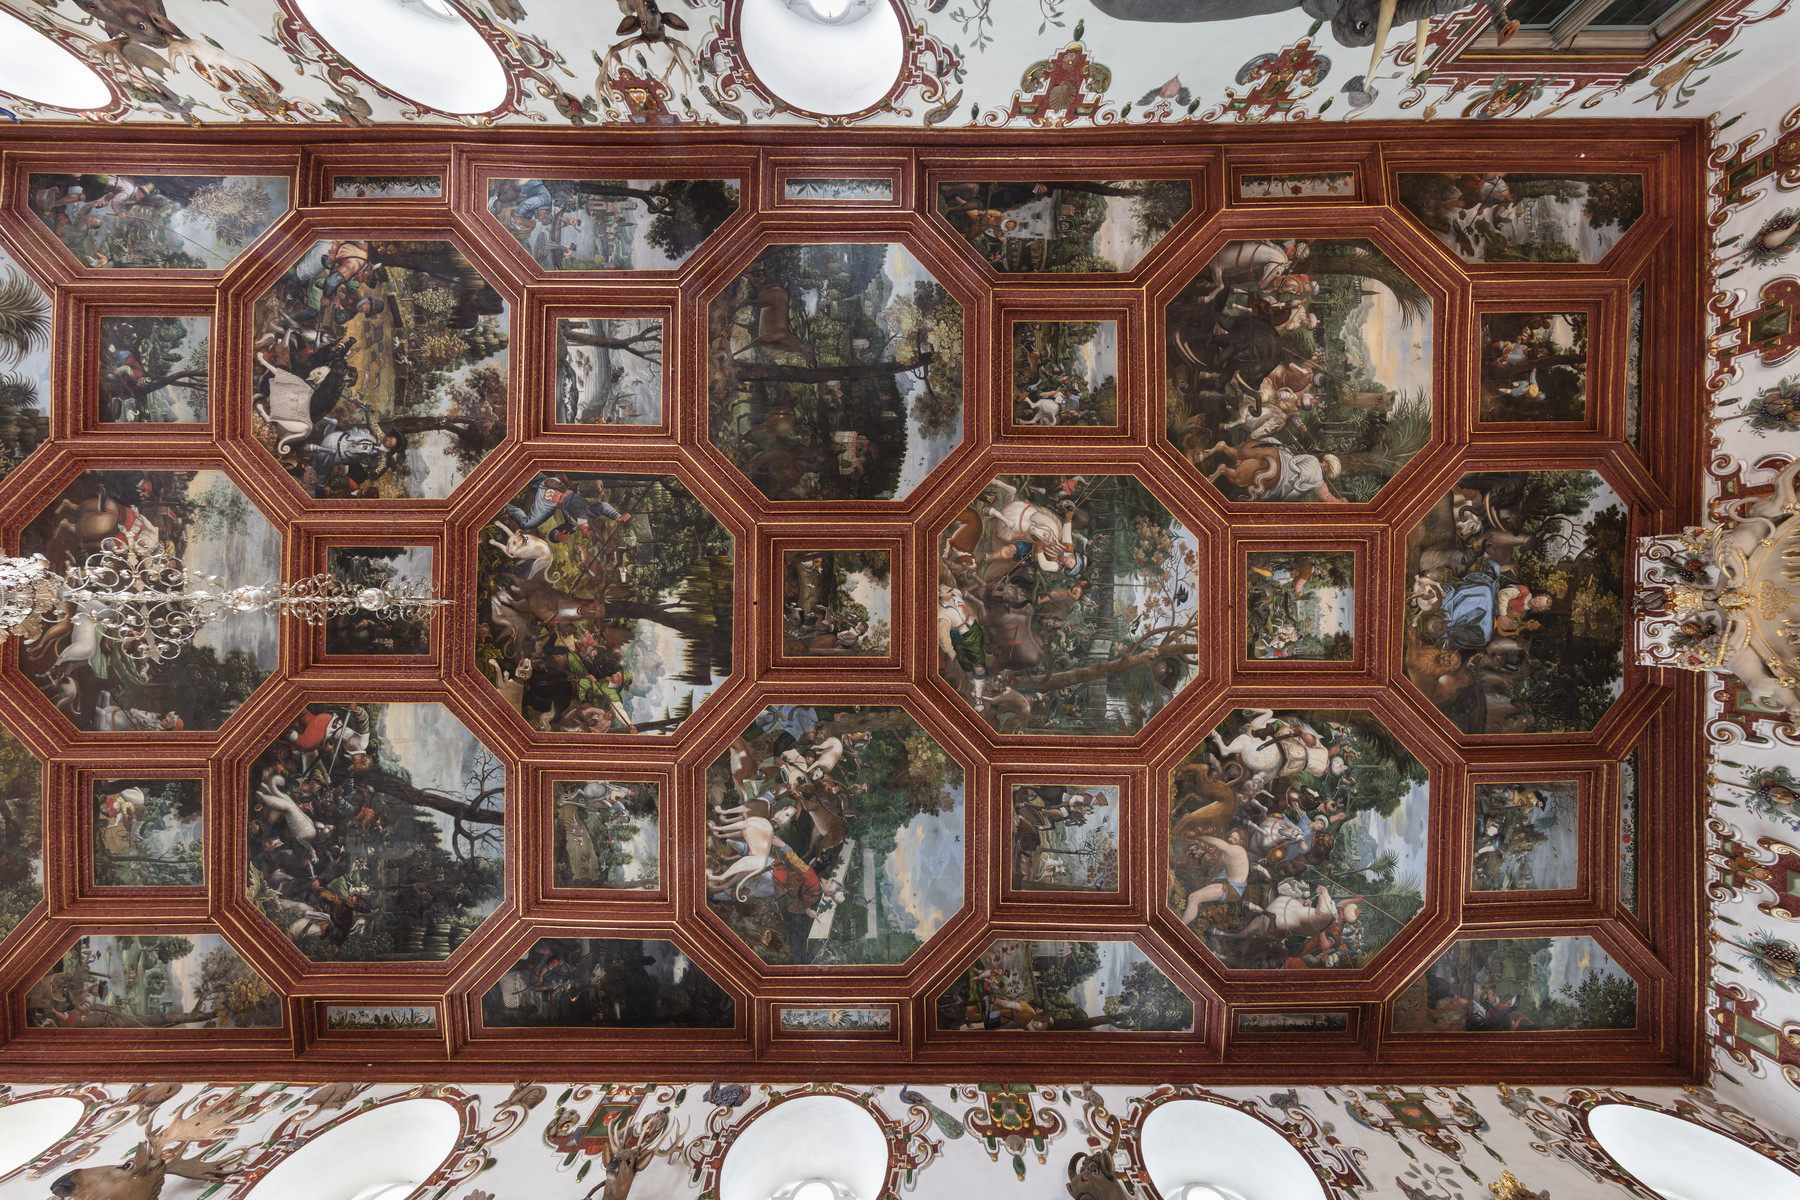
\includegraphics[height=10cm]{https://previous.bildindex.de/bilder/fmd10005870a.jpg}
  \caption{Ceiling Decoration of the Knights' Hall – Eastern Part of the Ceiling}
  \label{fig:{https://previous.bildindex.de/bilder/fmd10005870a.jpg}}
\end{figure}

\clearpage

\begin{figure}[H]    
  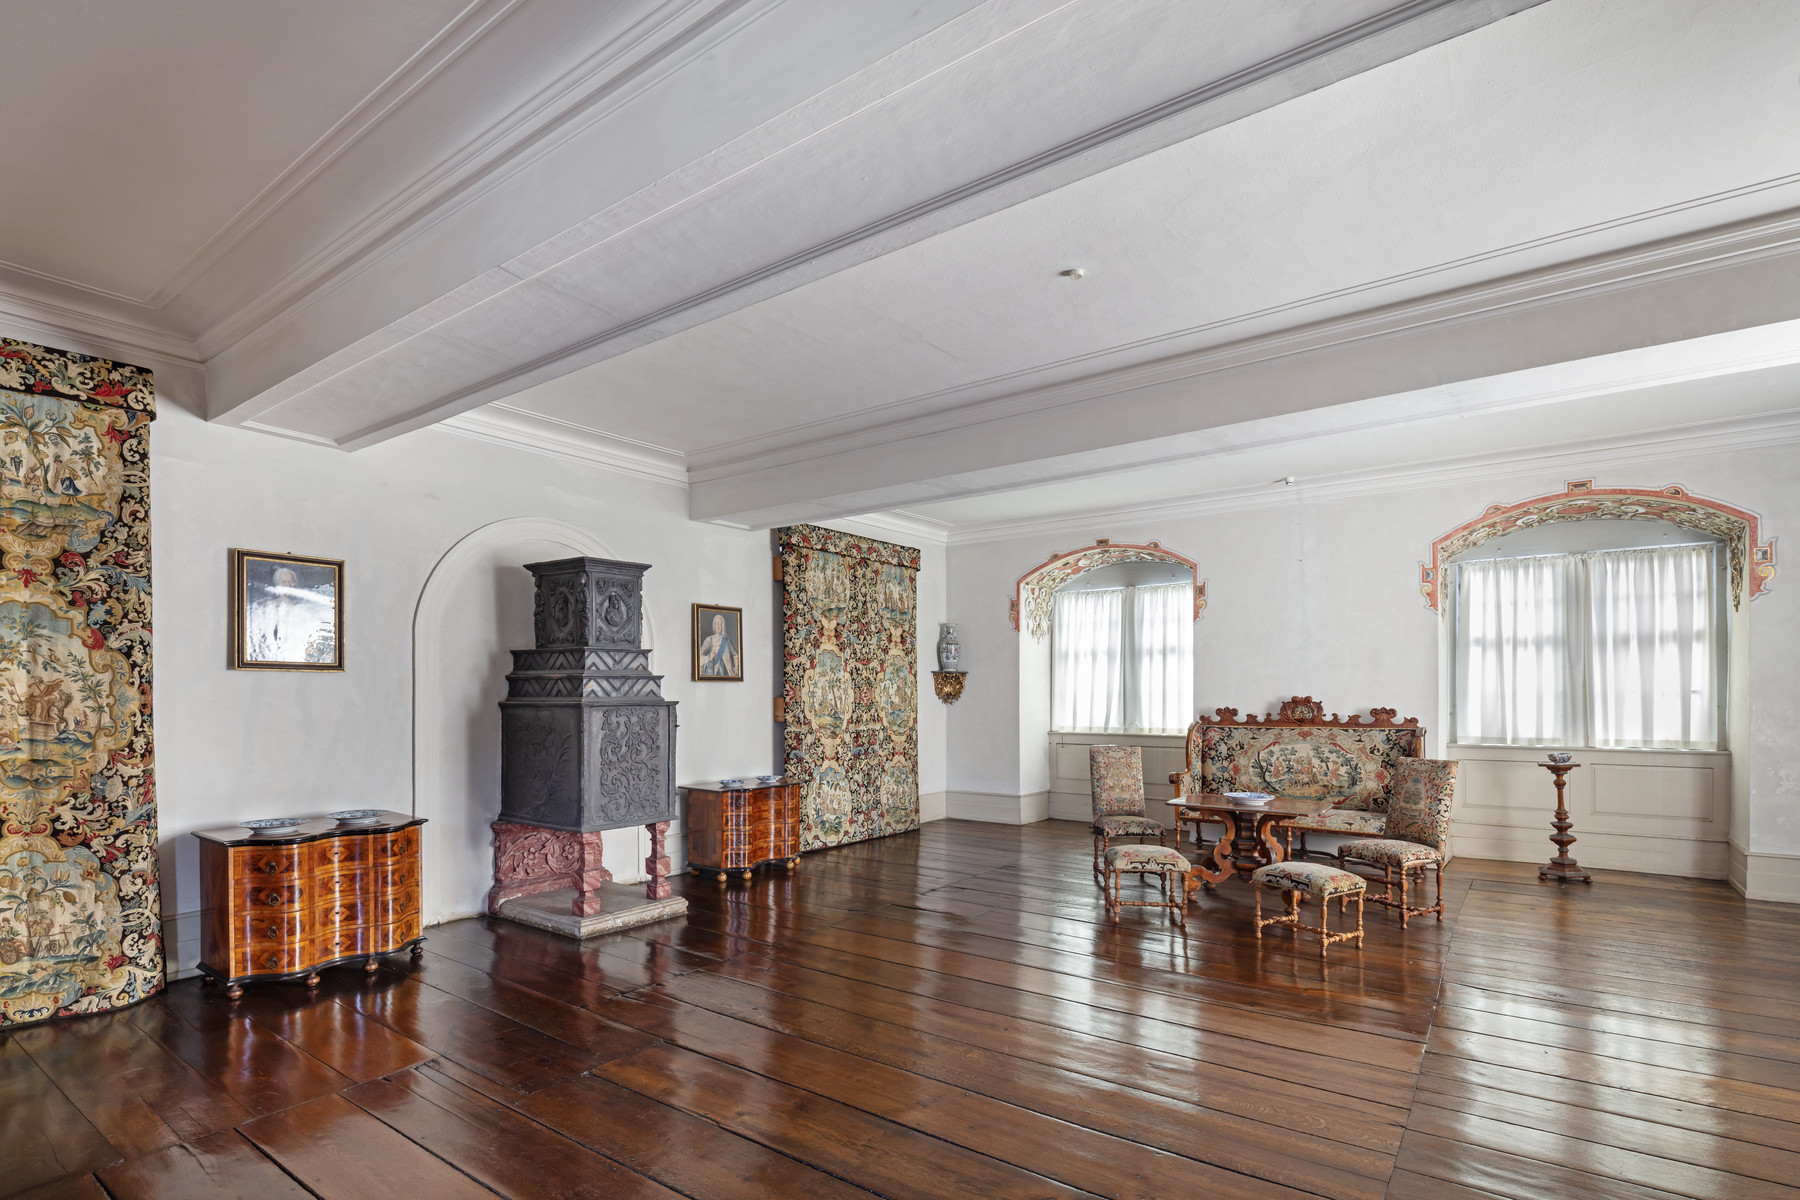
\includegraphics[height=10cm]{https://previous.bildindex.de/bilder/fmd10005852a.jpg}
  \caption{Einstige Tafelstube + Raum 69a – nach Südosten}
  \label{fig:{https://previous.bildindex.de/bilder/fmd10005852a.jpg}}
\end{figure}

\clearpage

\begin{figure}[H]    
  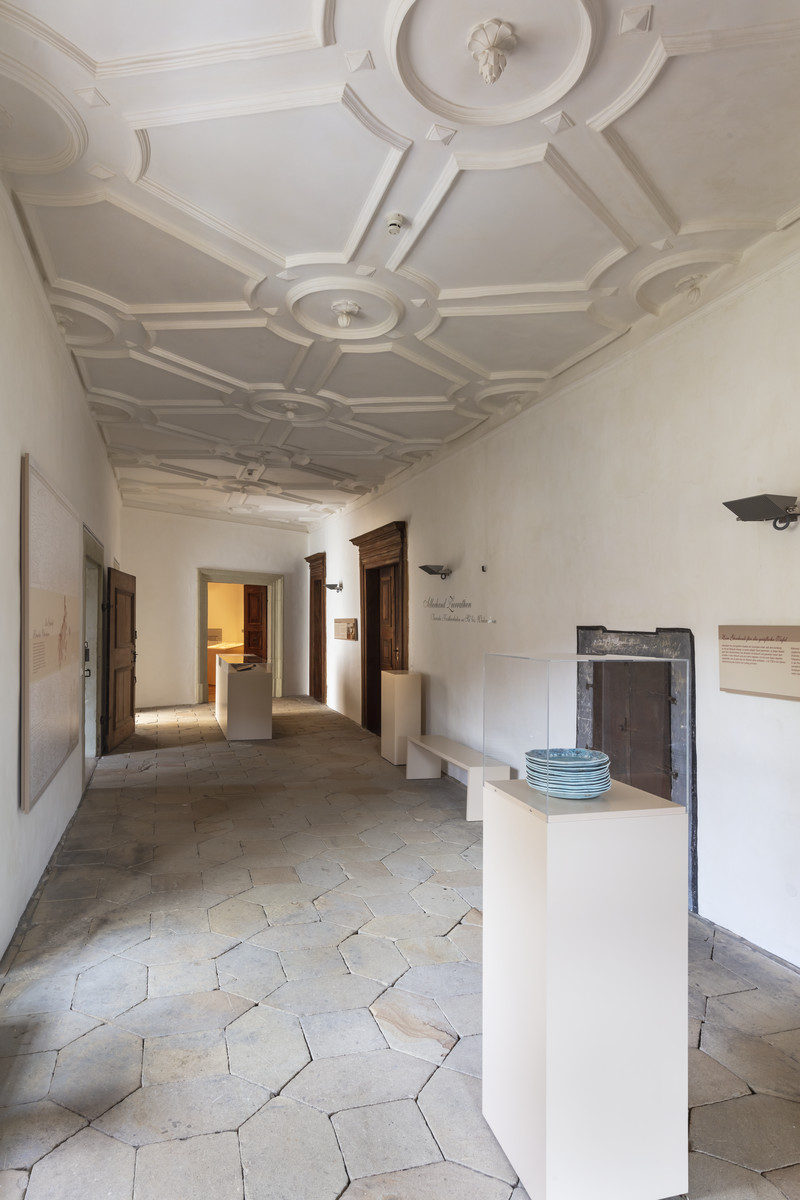
\includegraphics[height=10cm]{https://previous.bildindex.de/bilder/fmd10005855a.jpg}
  \caption{Der Saalbau Bild}
  \label{fig:{https://previous.bildindex.de/bilder/fmd10005855a.jpg}}
\end{figure}

\clearpage

\begin{figure}[H]    
  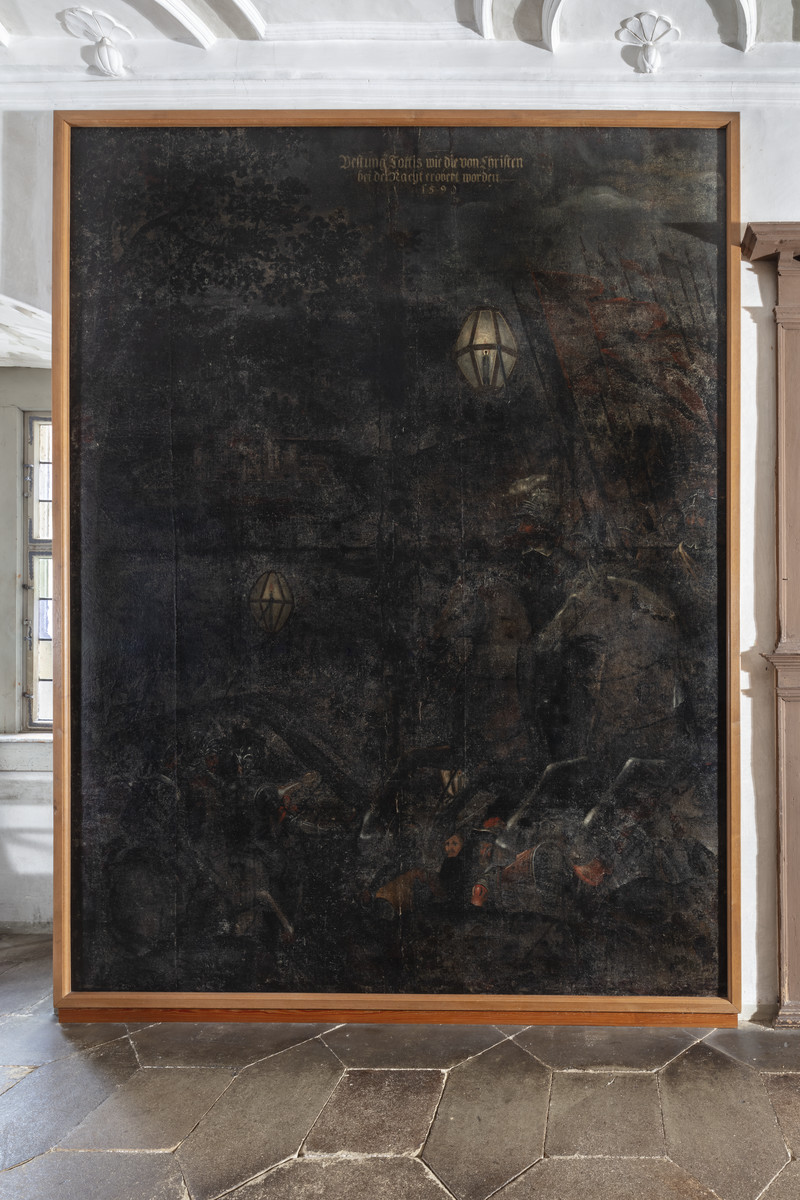
\includegraphics[height=10cm]{https://previous.bildindex.de/bilder/fmd10005851a.jpg}
  \caption{Eroberung der Festung Tottis – Gesamtansicht}
  \label{fig:{https://previous.bildindex.de/bilder/fmd10005851a.jpg}}
\end{figure}

\clearpage

\begin{figure}[H]    
  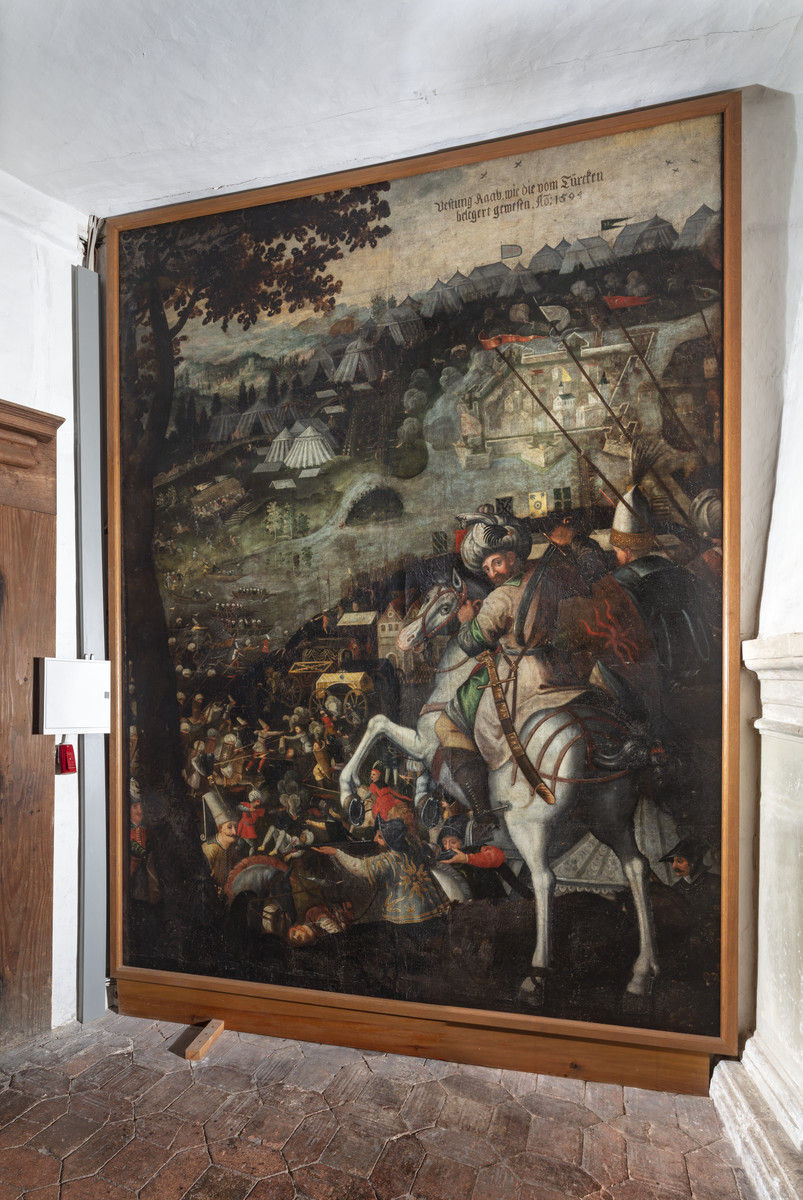
\includegraphics[height=10cm]{https://previous.bildindex.de/bilder/fmd10005843a.jpg}
  \caption{Belagerung der Festung Raab – Gesamtansicht}
  \label{fig:{https://previous.bildindex.de/bilder/fmd10005843a.jpg}}
\end{figure}

\clearpage

\begin{figure}[H]    
  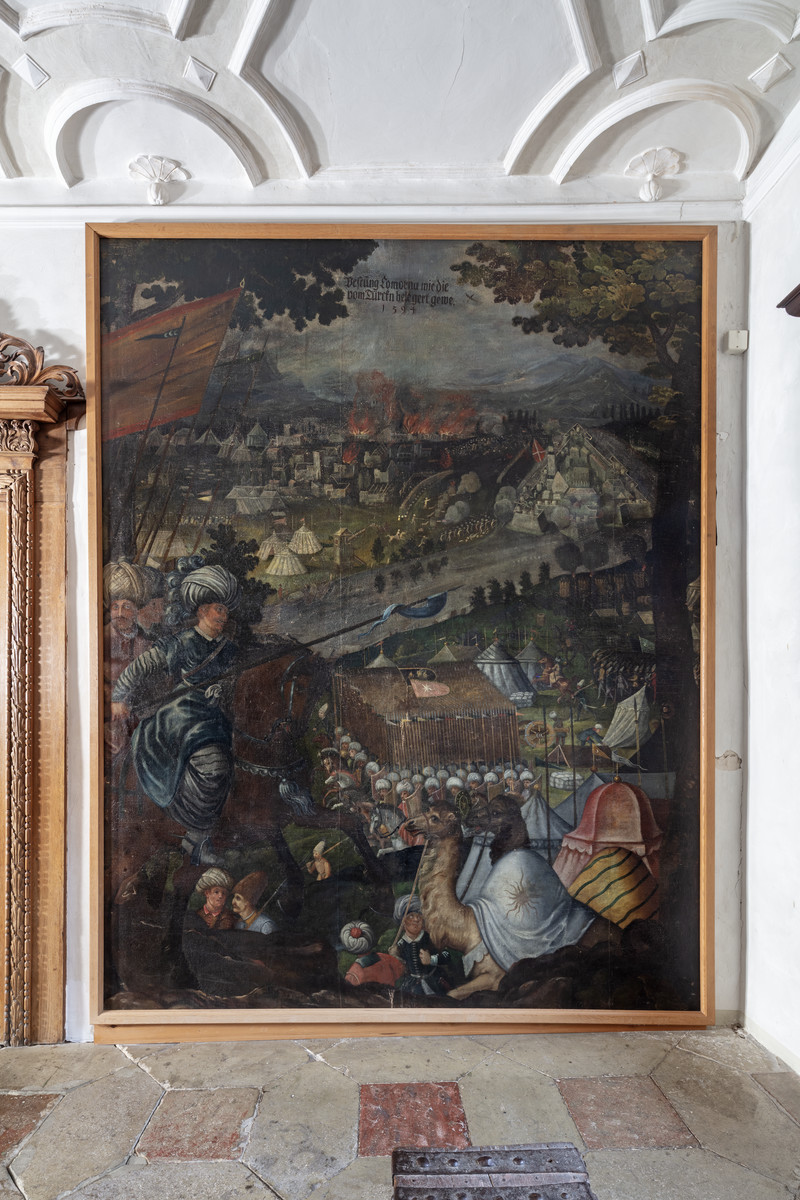
\includegraphics[height=10cm]{https://previous.bildindex.de/bilder/fmd10005850a.jpg}
  \caption{Belagerung der Festung Comorna – Gesamtansicht}
  \label{fig:{https://previous.bildindex.de/bilder/fmd10005850a.jpg}}
\end{figure}

\clearpage

\begin{figure}[H]    
  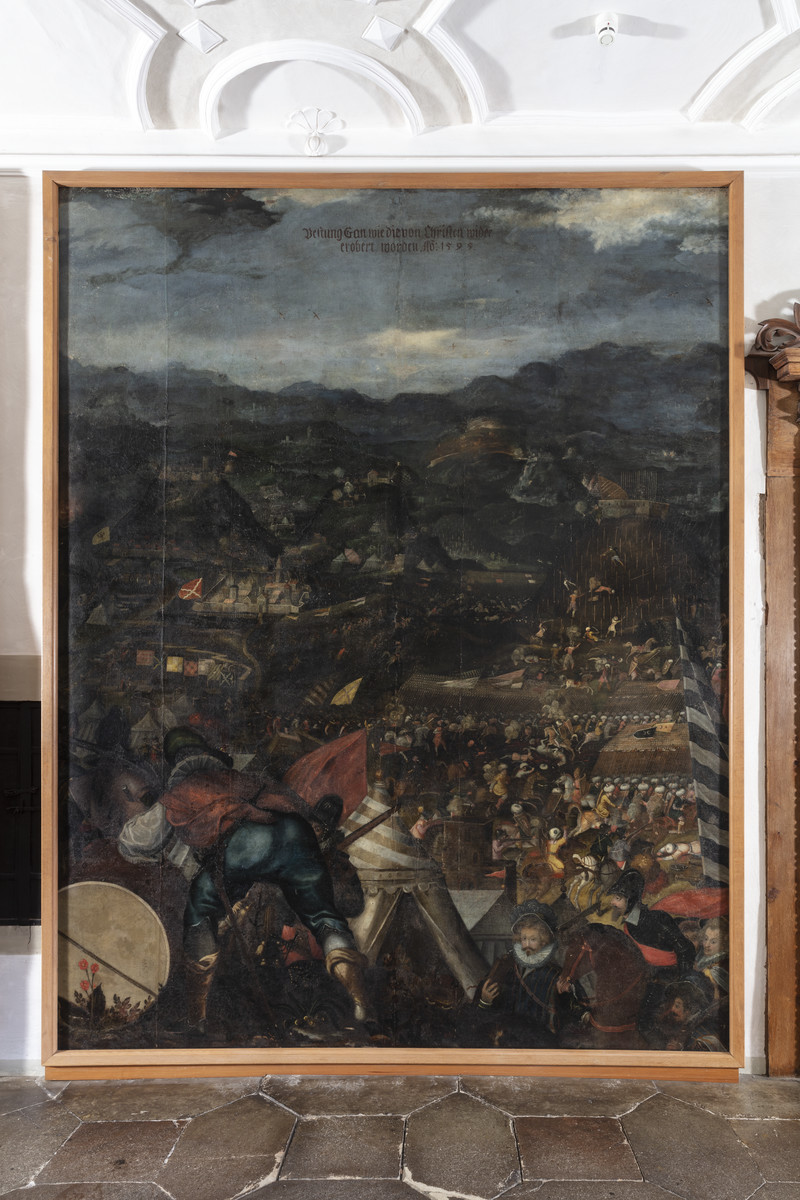
\includegraphics[height=10cm]{https://previous.bildindex.de/bilder/fmd10005848a.jpg}
  \caption{Eroberung der Festung Gran – Gesamtansicht}
  \label{fig:{https://previous.bildindex.de/bilder/fmd10005848a.jpg}}
\end{figure}

\clearpage

\begin{figure}[H]    
  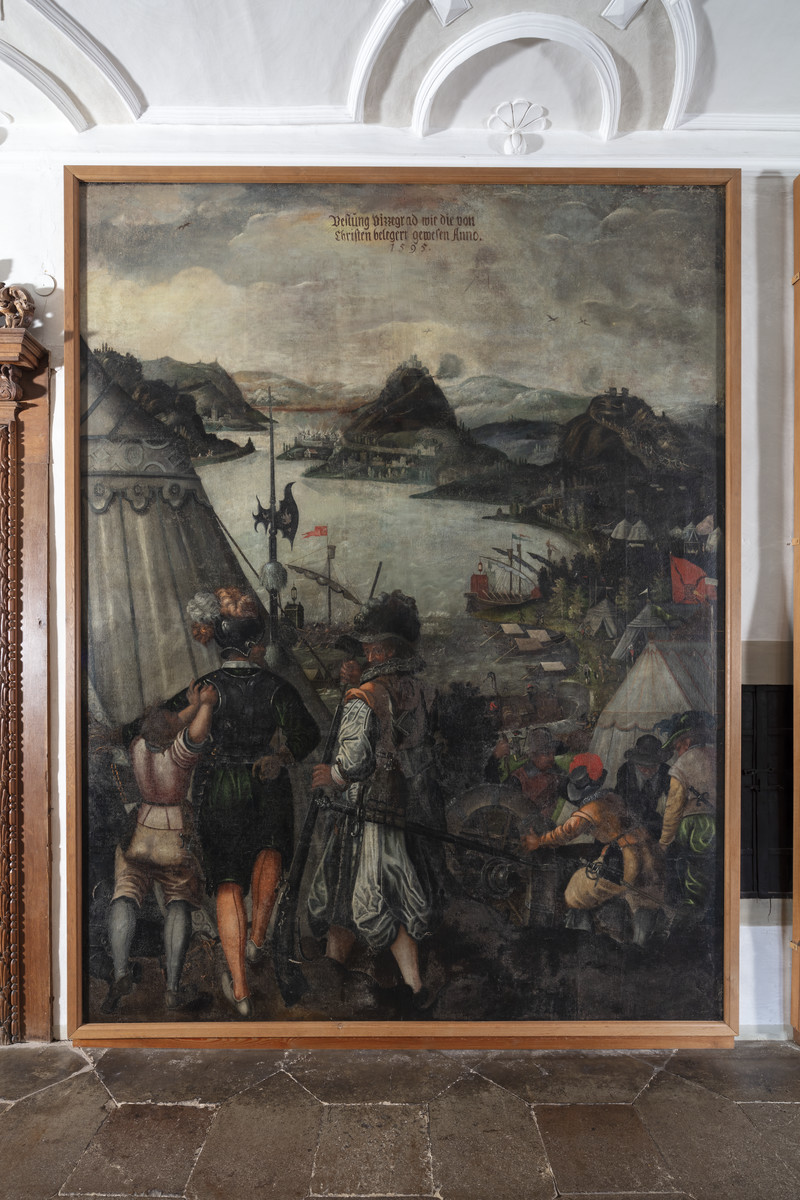
\includegraphics[height=10cm]{https://previous.bildindex.de/bilder/fmd10005840a.jpg}
  \caption{Belagerung der Festung von Visegrád – Gesamtansicht}
  \label{fig:{https://previous.bildindex.de/bilder/fmd10005840a.jpg}}
\end{figure}

\clearpage

\begin{figure}[H]    
  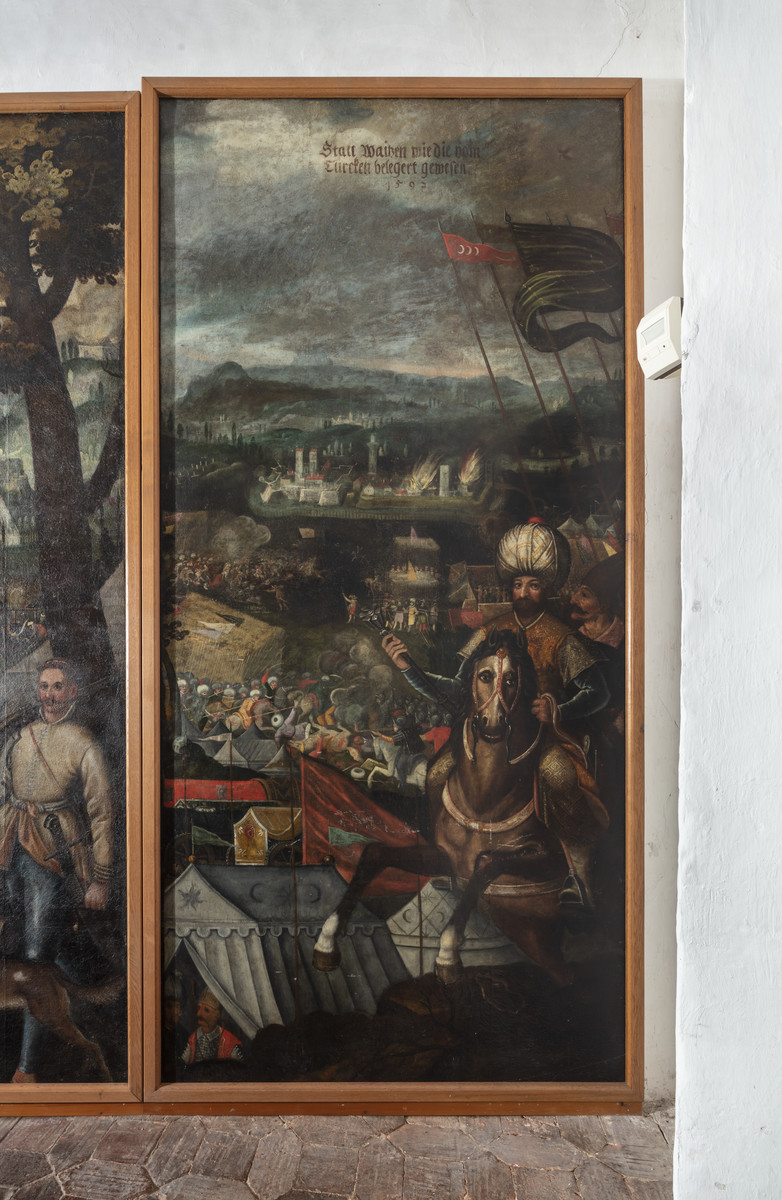
\includegraphics[height=10cm]{https://previous.bildindex.de/bilder/fmd10005842a.jpg}
  \caption{Belagerung der Stadt Waitzen – Gesamtansicht}
  \label{fig:{https://previous.bildindex.de/bilder/fmd10005842a.jpg}}
\end{figure}

\clearpage

\begin{figure}[H]    
  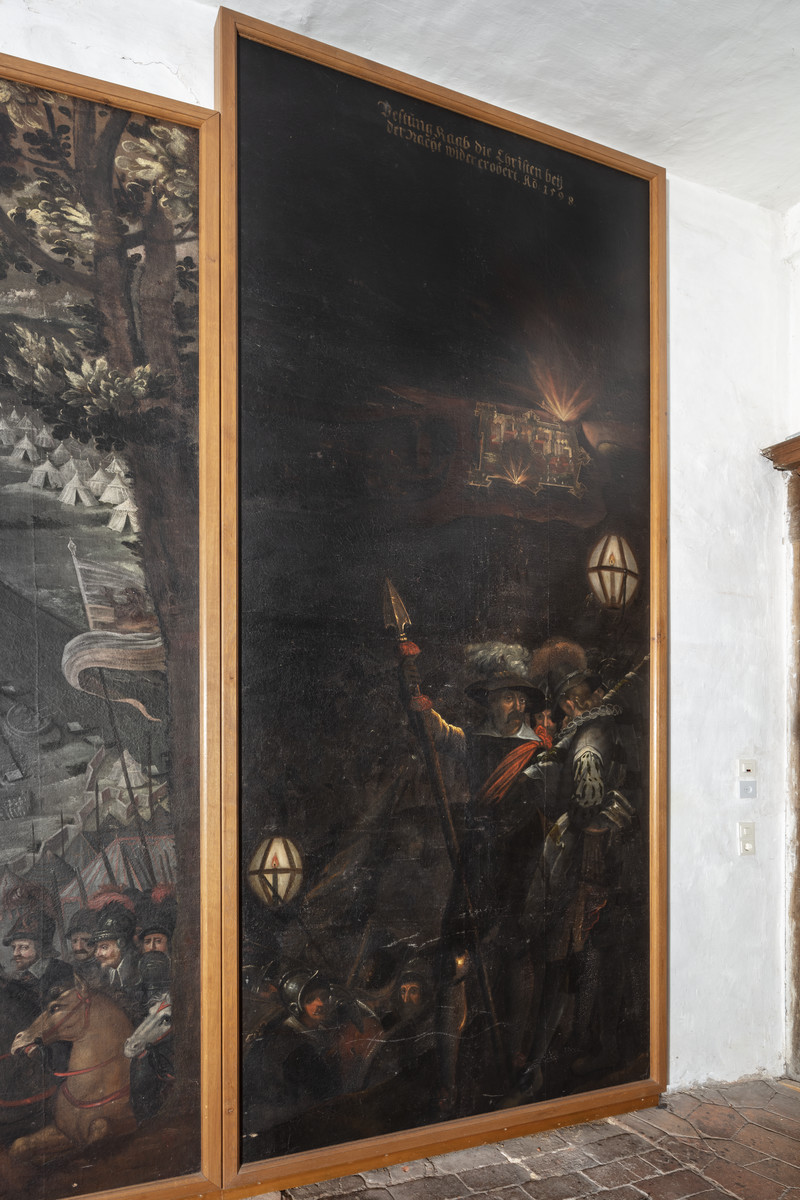
\includegraphics[height=10cm]{https://previous.bildindex.de/bilder/fmd10005846a.jpg}
  \caption{Wiedereroberung der Festung Raab – Gesamtansicht}
  \label{fig:{https://previous.bildindex.de/bilder/fmd10005846a.jpg}}
\end{figure}

\clearpage

\begin{figure}[H]    
  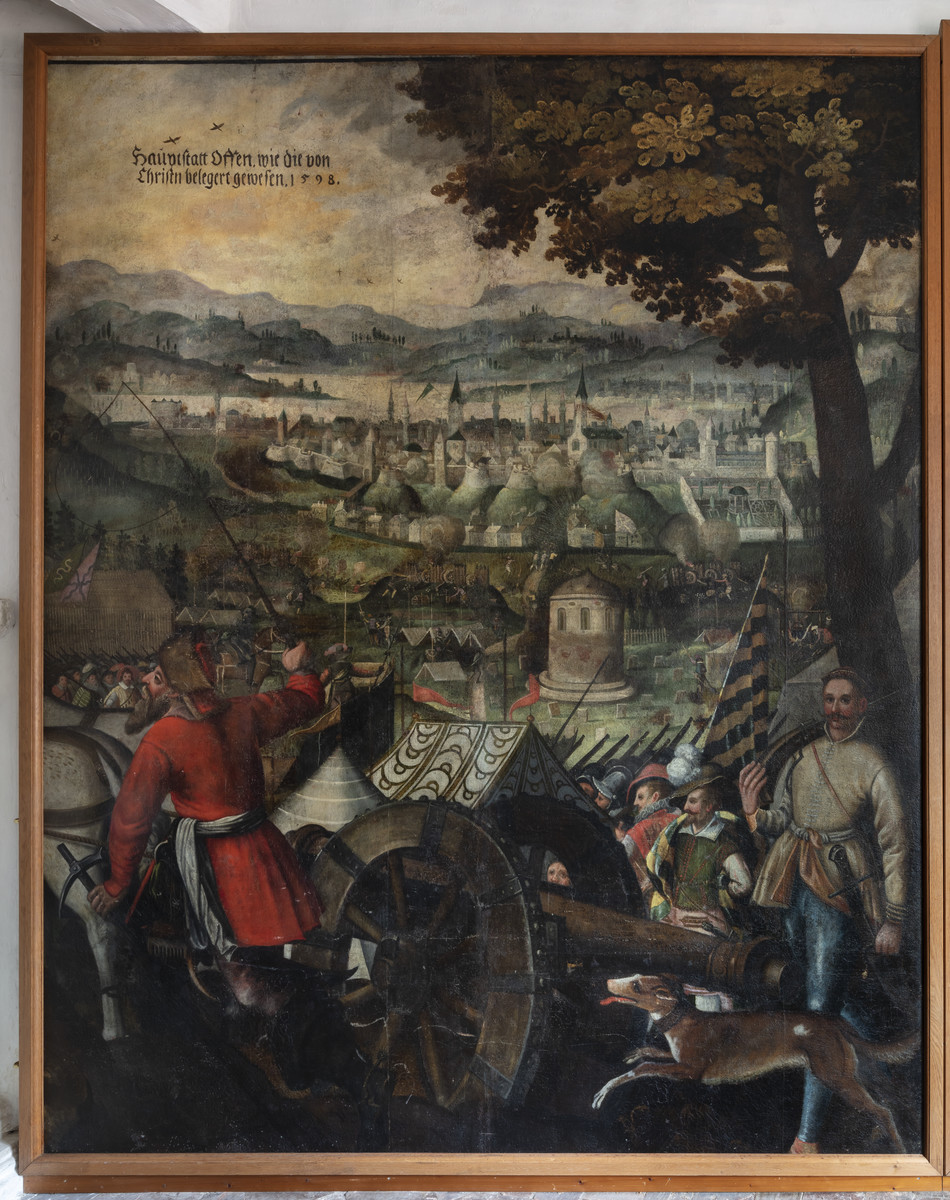
\includegraphics[height=10cm]{https://previous.bildindex.de/bilder/fmd10005847a.jpg}
  \caption{Belagerung der Stadt Ofen im Jahr 1598 – Gesamtansicht}
  \label{fig:{https://previous.bildindex.de/bilder/fmd10005847a.jpg}}
\end{figure}

\clearpage

\begin{figure}[H]    
  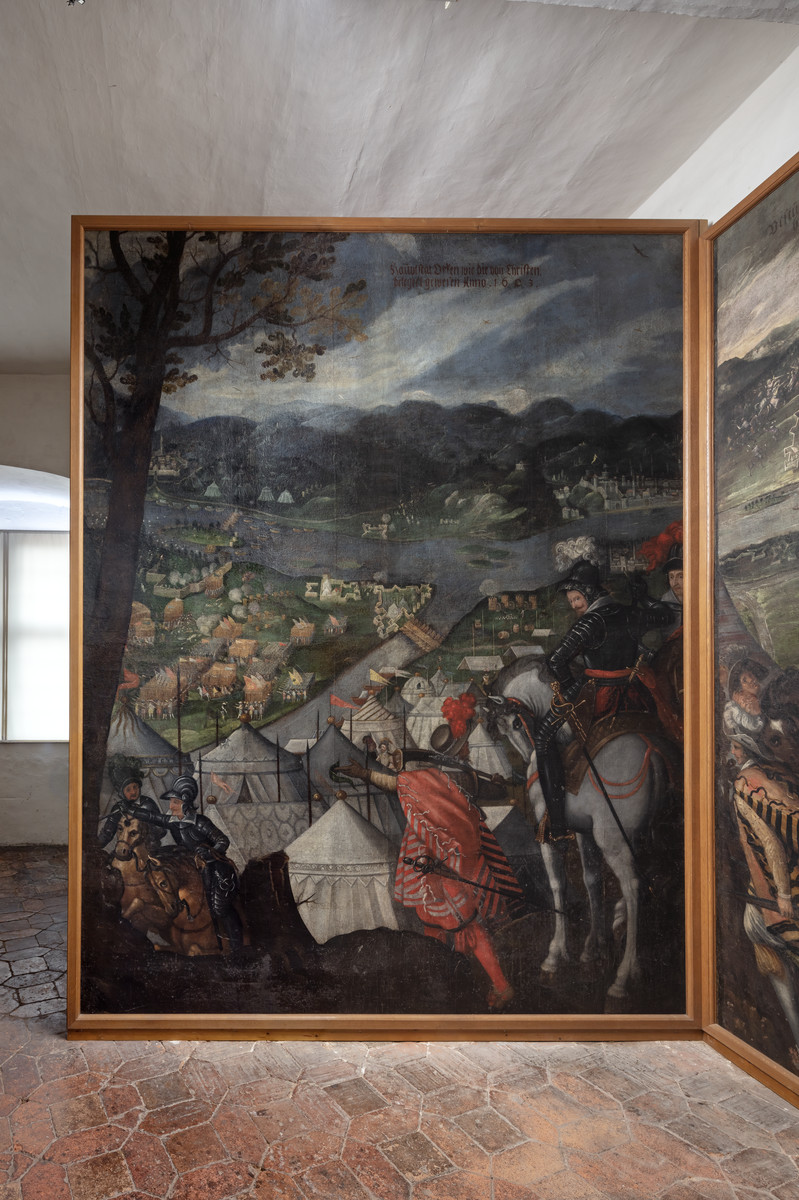
\includegraphics[height=10cm]{https://previous.bildindex.de/bilder/fmd10005844a.jpg}
  \caption{Belagerung der Stadt Ofen im Jahr 1603 – Gesamtansicht}
  \label{fig:{https://previous.bildindex.de/bilder/fmd10005844a.jpg}}
\end{figure}

\clearpage

\begin{figure}[H]    
  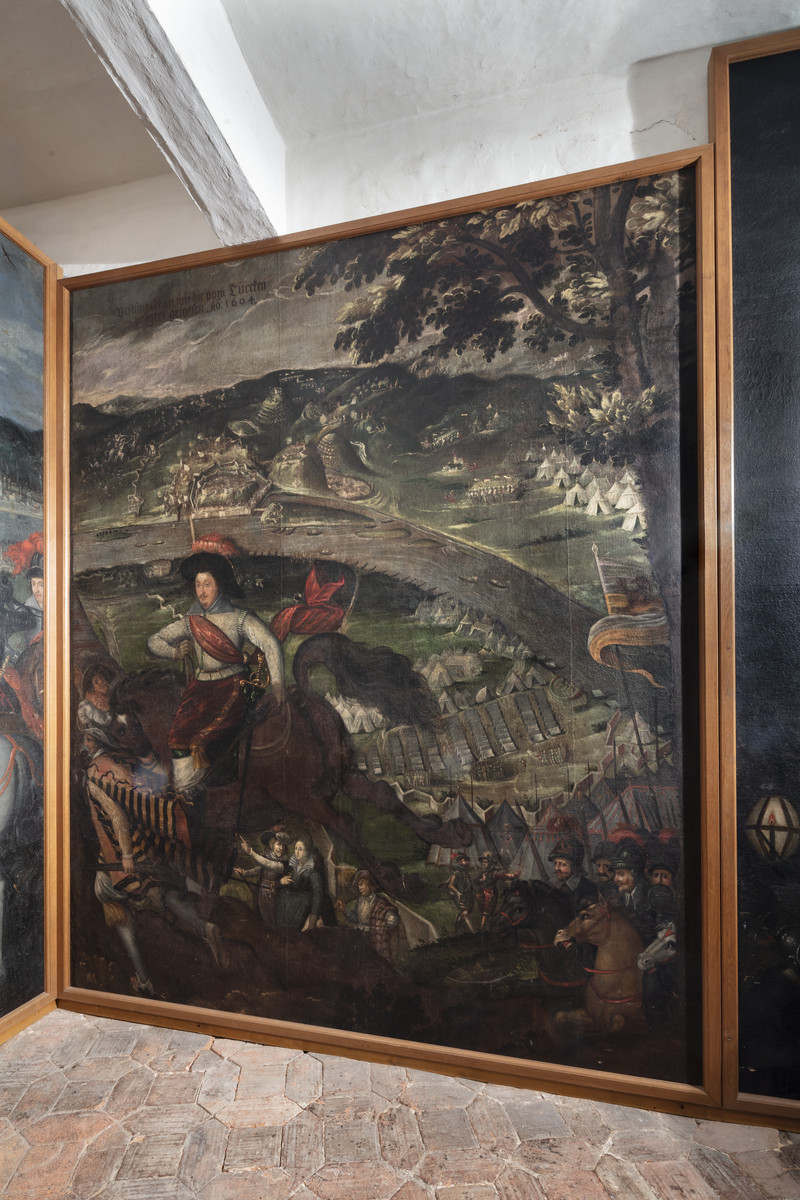
\includegraphics[height=10cm]{https://previous.bildindex.de/bilder/fmd10005845a.jpg}
  \caption{Belagerung der Festung Gran – Gesamtansicht (Anno 1604)}
  \label{fig:{https://previous.bildindex.de/bilder/fmd10005845a.jpg}}
\end{figure}

\clearpage

\begin{figure}[H]    
  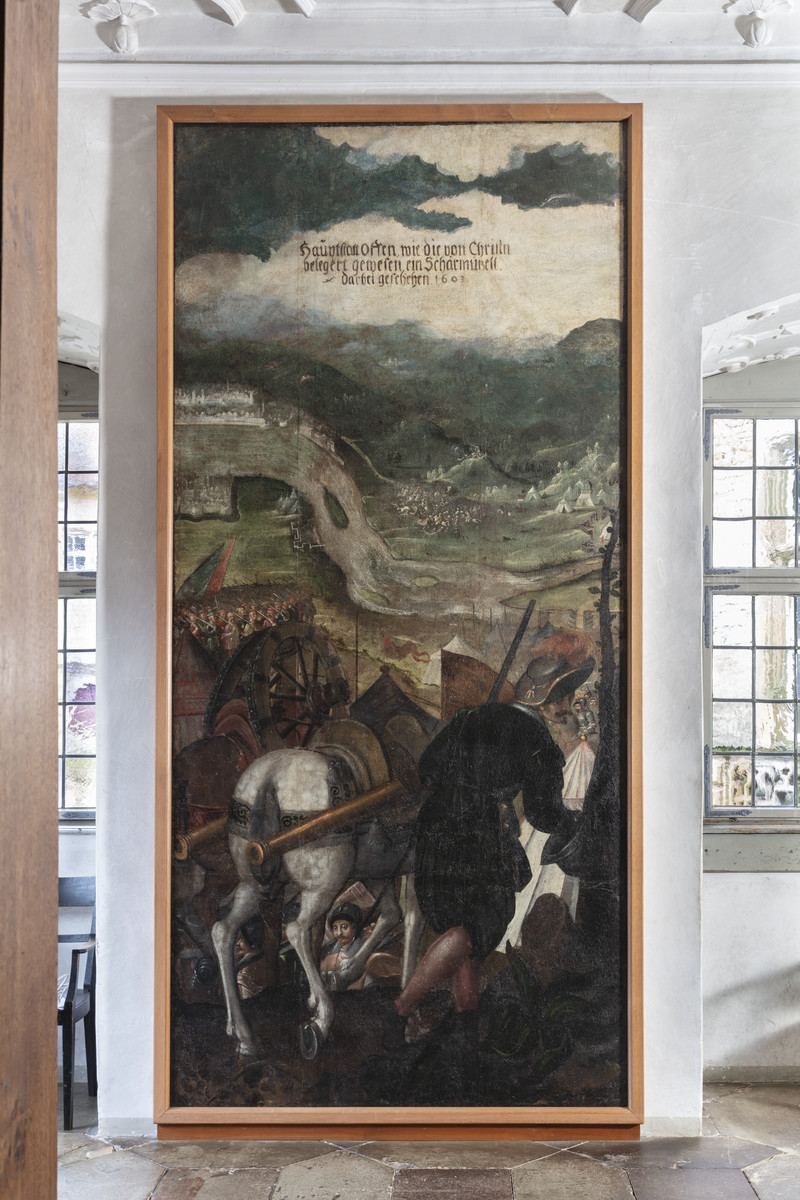
\includegraphics[height=10cm]{https://previous.bildindex.de/bilder/fmd10005849a.jpg}
  \caption{Scharmützel bei der Belagerung der Stadt Ofen im Jahr 1603 – Gesamtansicht}
  \label{fig:{https://previous.bildindex.de/bilder/fmd10005849a.jpg}}
\end{figure}

\clearpage

\begin{figure}[H]    
  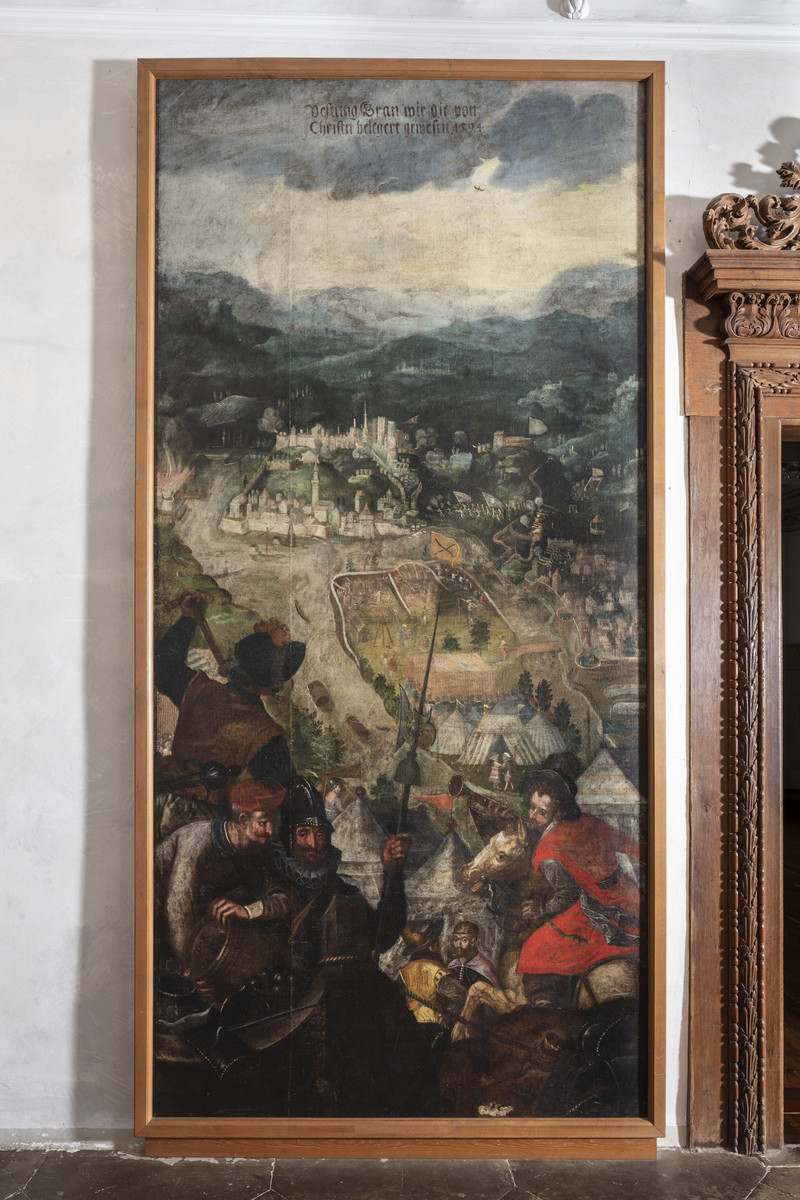
\includegraphics[height=10cm]{https://previous.bildindex.de/bilder/fmd10005841a.jpg}
  \caption{Belagerung der Festung Gran – Gesamtansicht (1594)}
  \label{fig:{https://previous.bildindex.de/bilder/fmd10005841a.jpg}}
\end{figure}

\clearpage

\begin{figure}[H]    
  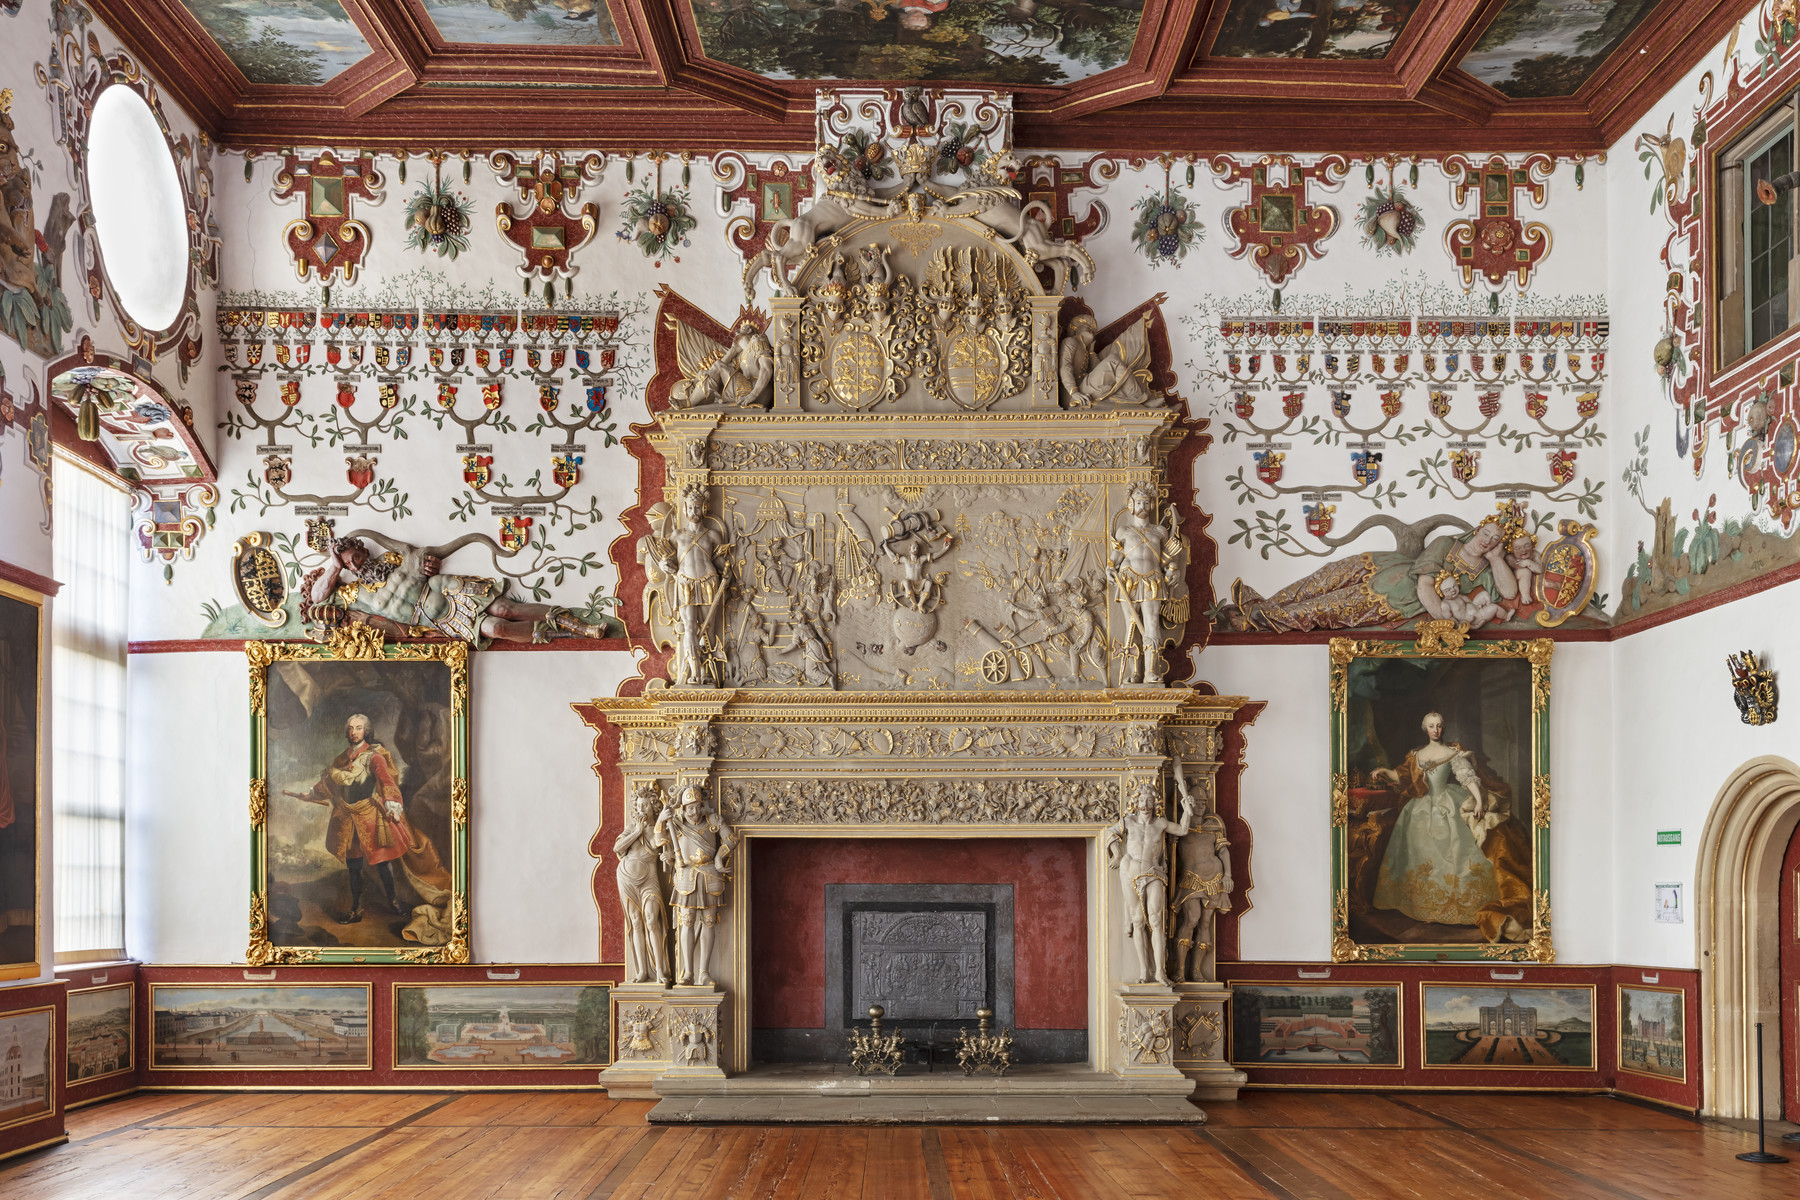
\includegraphics[height=10cm]{https://previous.bildindex.de/bilder/fmd10005861a.jpg}
  \caption{Die barocken Schloss- und Gartenveduten bild}
  \label{fig:{https://previous.bildindex.de/bilder/fmd10005861a.jpg}}
\end{figure}

\clearpage

\begin{figure}[H]    
  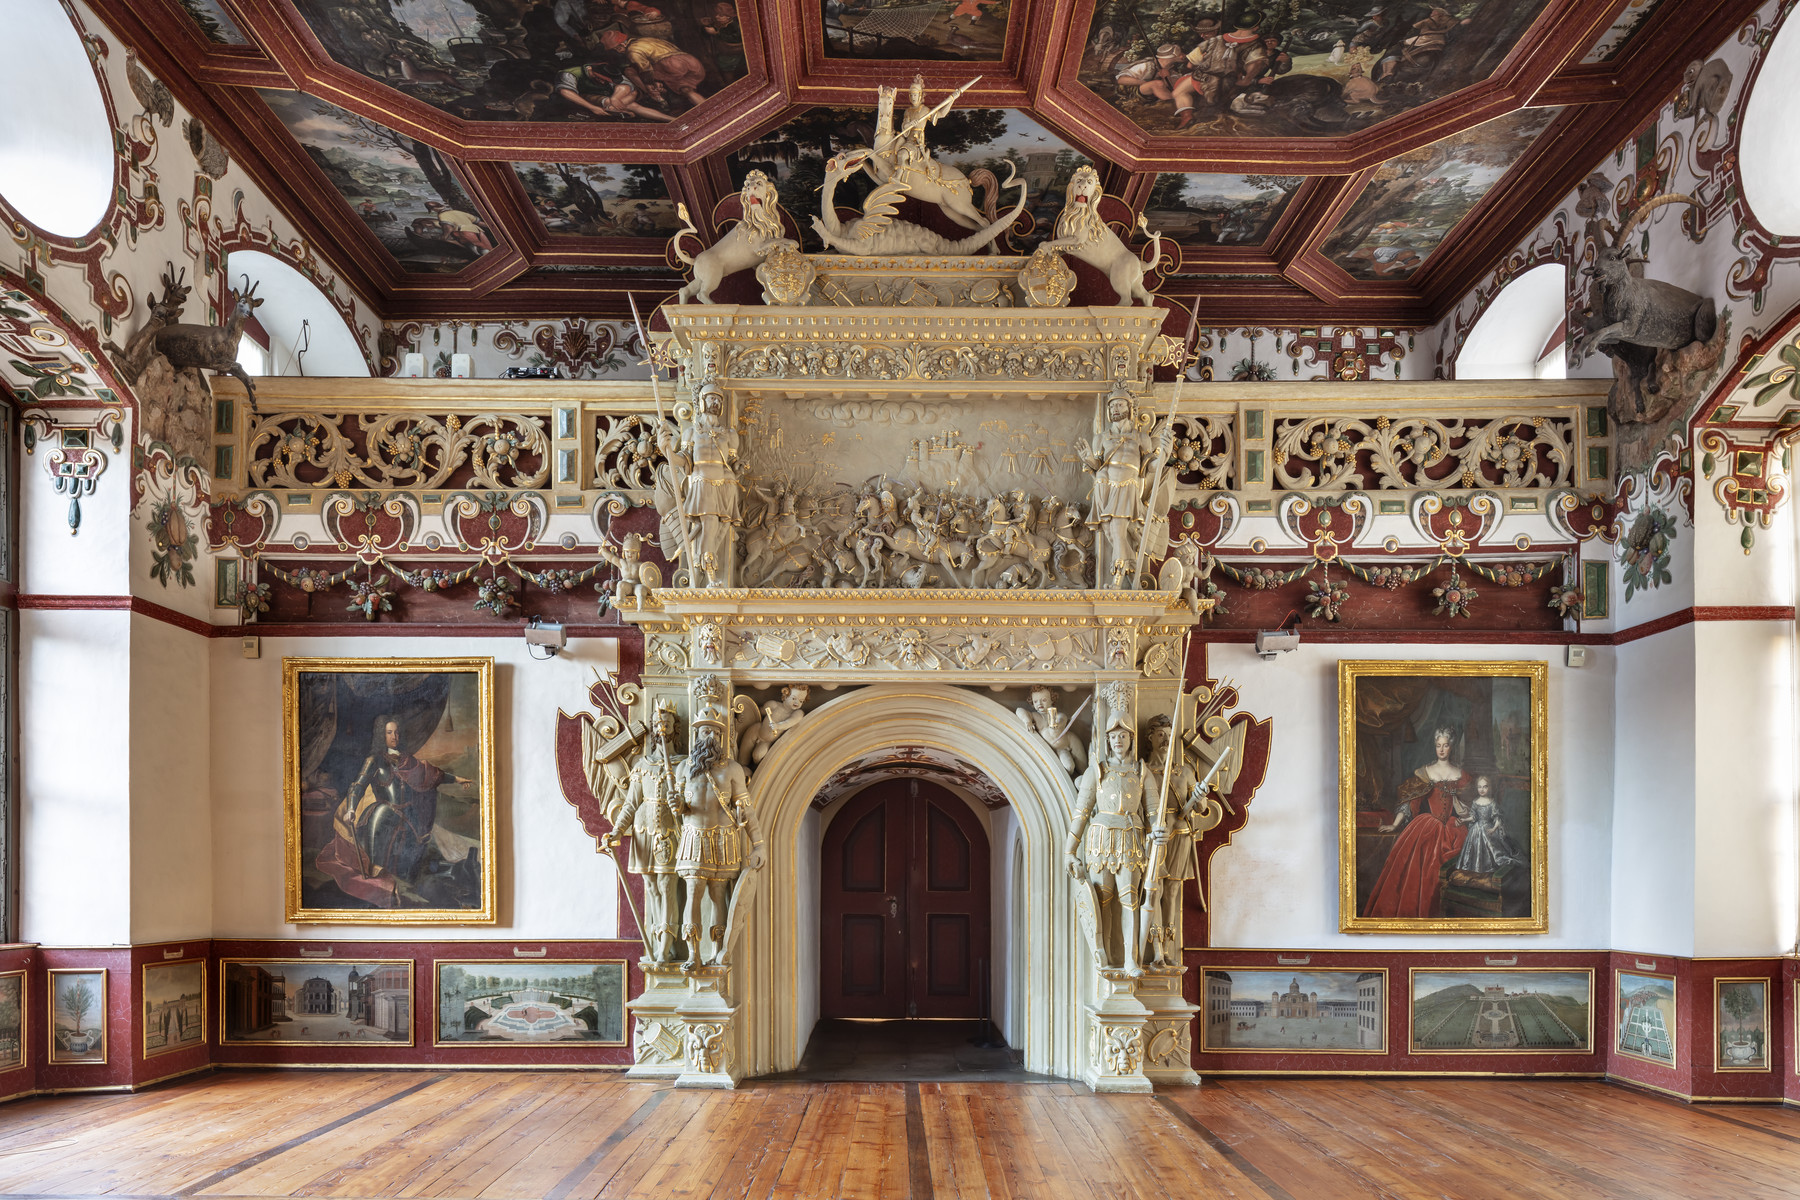
\includegraphics[height=10cm]{https://previous.bildindex.de/bilder/fmd10005863a.jpg}
  \caption{Die barocken Schloss- und Gartenveduten bild 2}
  \label{fig:{https://previous.bildindex.de/bilder/fmd10005863a.jpg}}
\end{figure}

\clearpage

\begin{figure}[H]    
  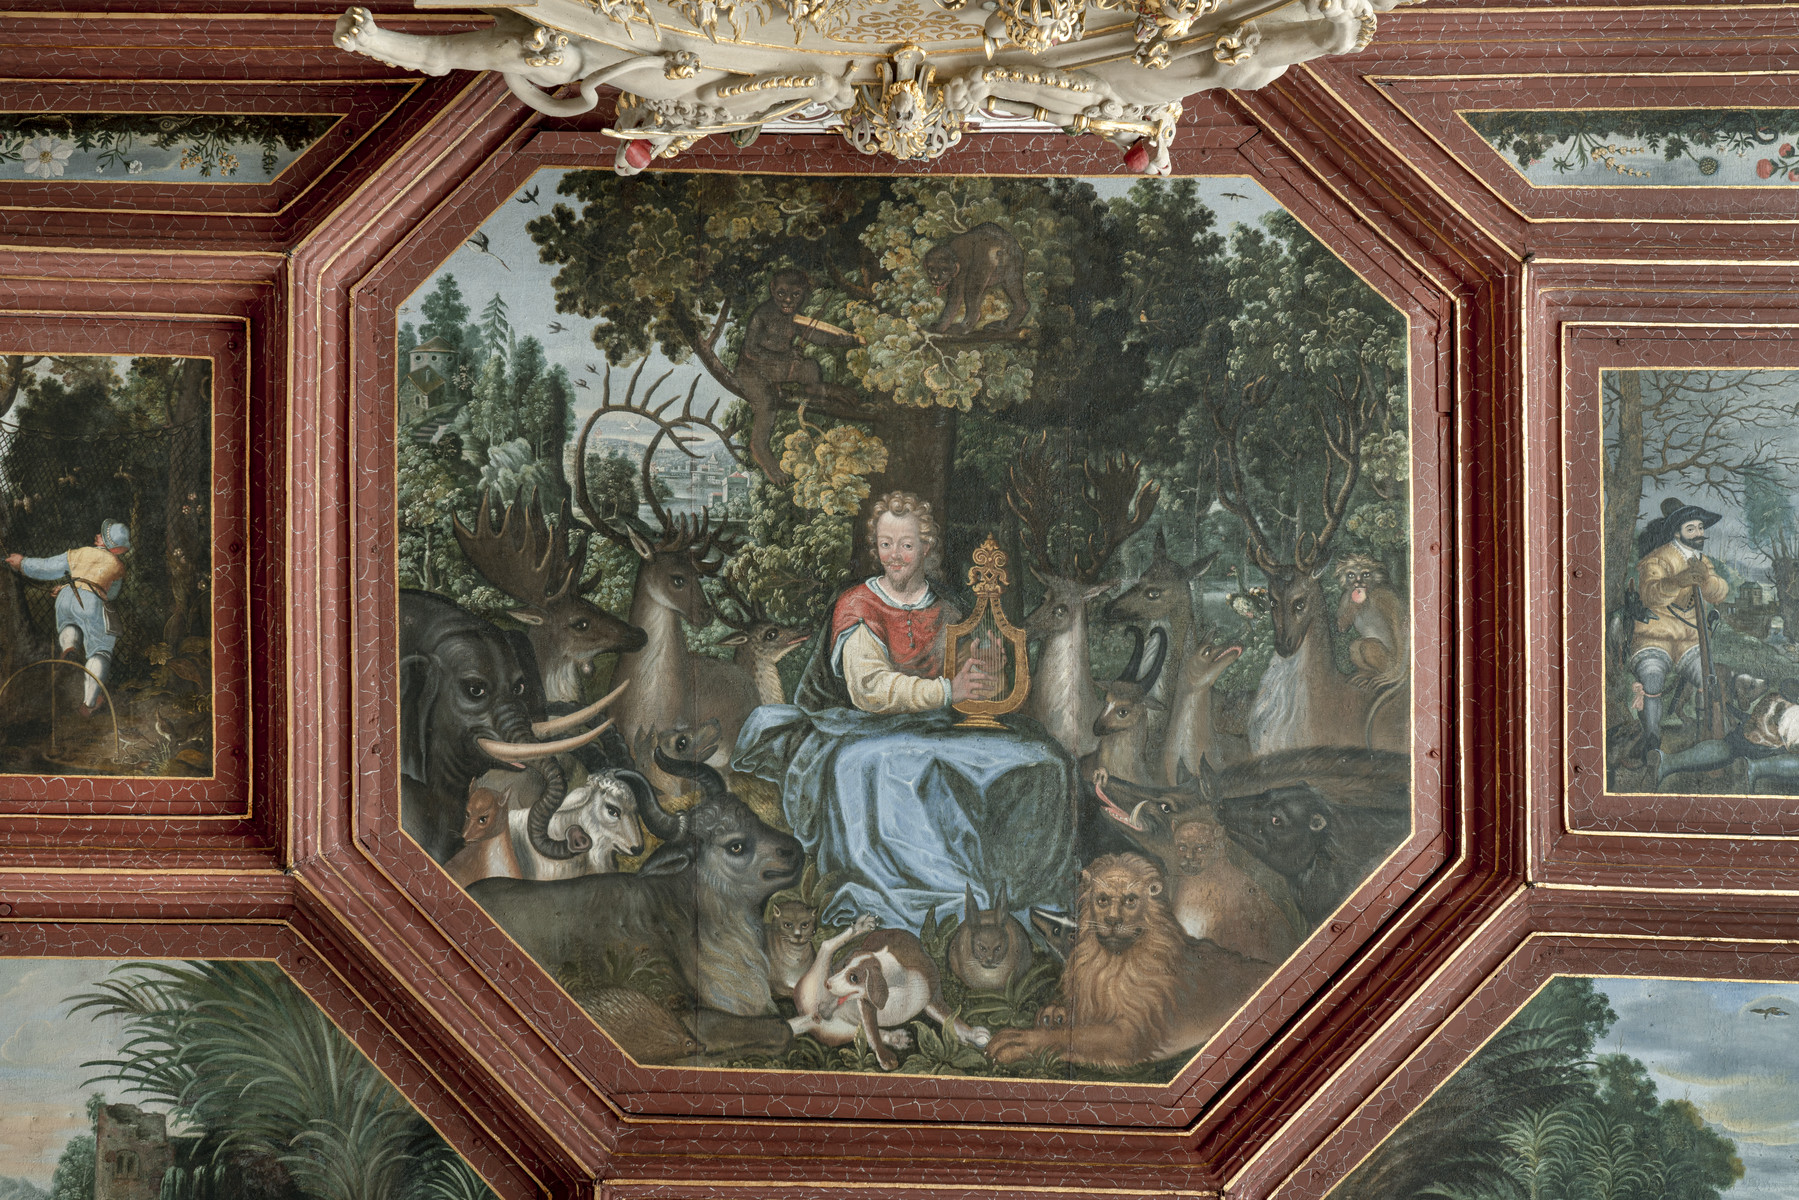
\includegraphics[height=10cm]{https://previous.bildindex.de/bilder/fmd10024323a.jpg}
  \caption{Orpheus with the lyre and the animals under a tree}
  \label{fig:{https://previous.bildindex.de/bilder/fmd10024323a.jpg}}
\end{figure}

\clearpage

\begin{figure}[H]    
  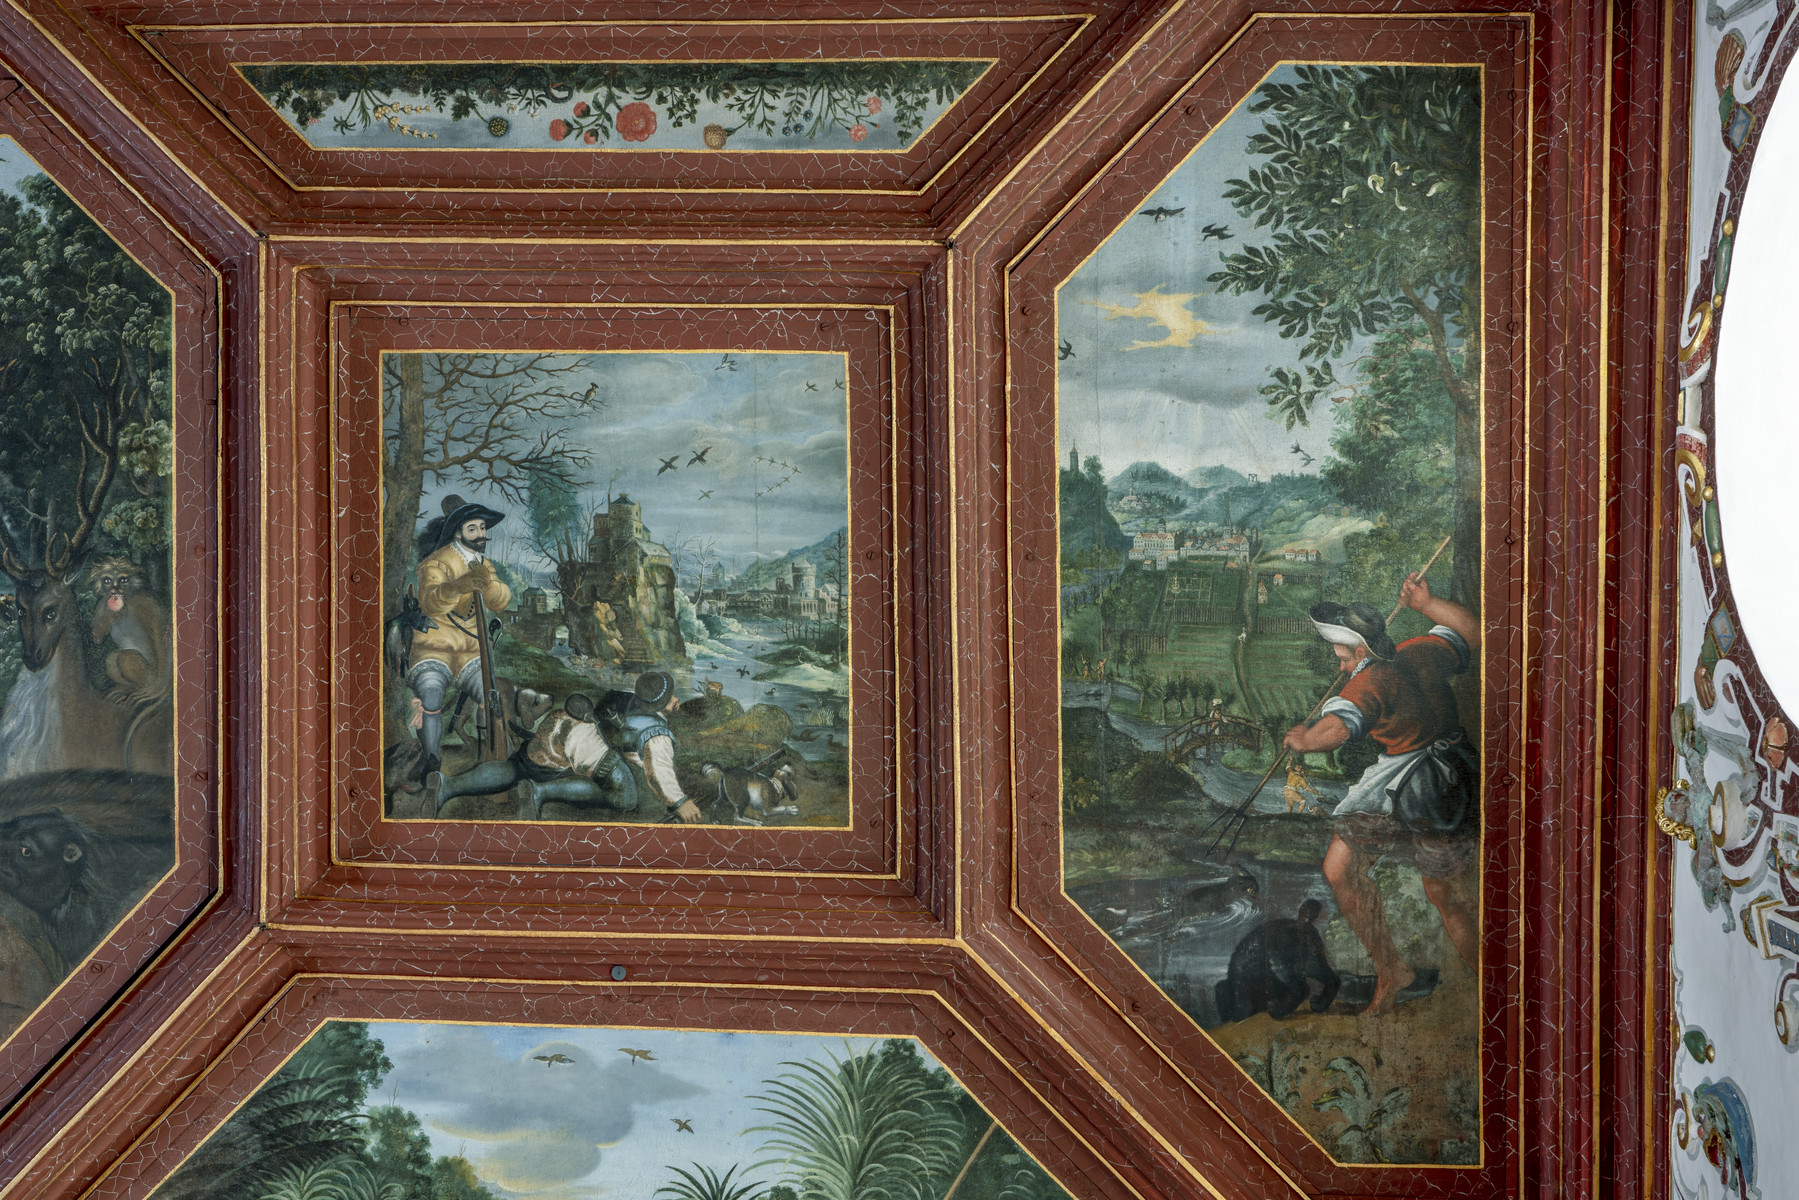
\includegraphics[height=10cm]{https://previous.bildindex.de/bilder/fmd10024324a.jpg}
  \caption{Otter catching, with Weikersheim Castle in the background – on the left, duck hunting, on the right, otter catching}
  \label{fig:{https://previous.bildindex.de/bilder/fmd10024324a.jpg}}
\end{figure}

\clearpage

\begin{figure}[H]    
  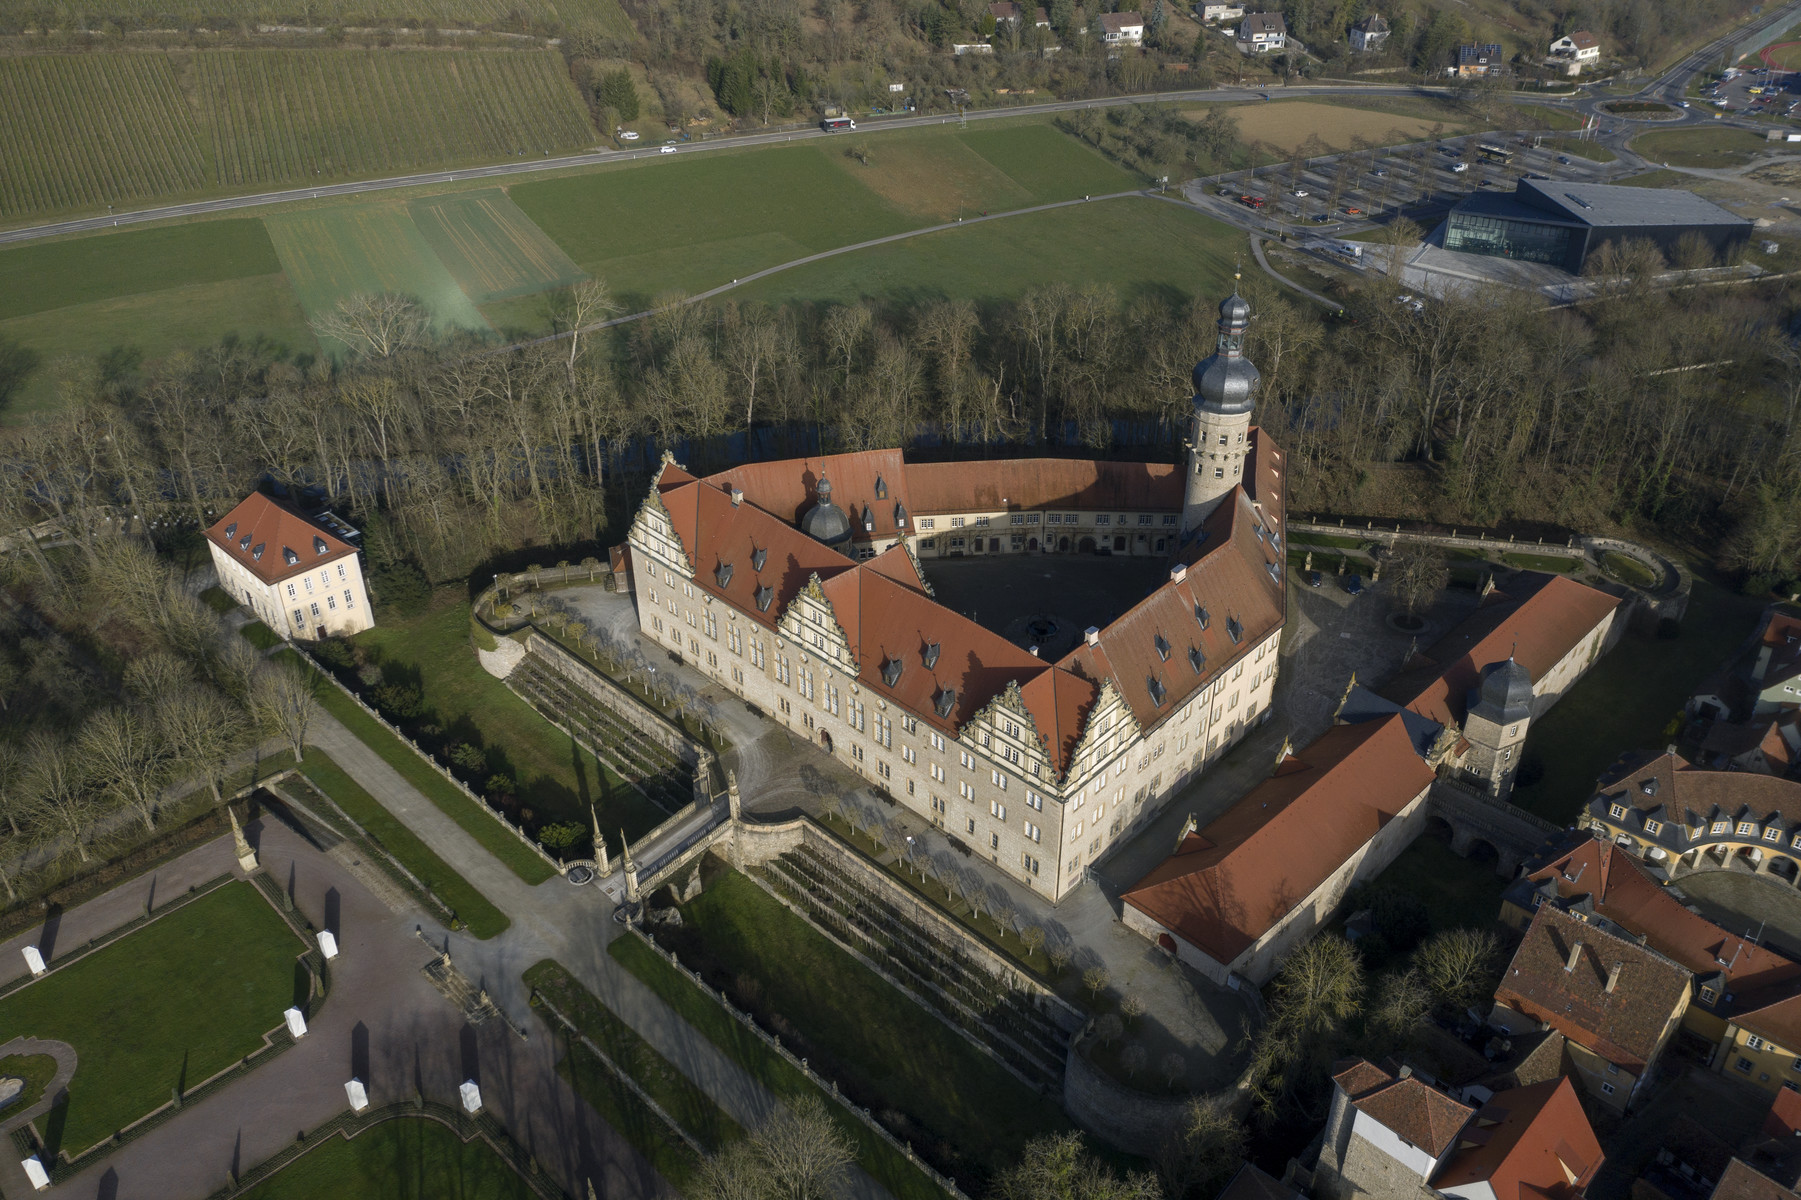
\includegraphics[height=10cm]{https://previous.bildindex.de/bilder/fmd10024322a.jpg}
  \caption{Schloss}
  \label{fig:{https://previous.bildindex.de/bilder/fmd10024322a.jpg}}
\end{figure}

\clearpage

\begin{figure}[H]    
  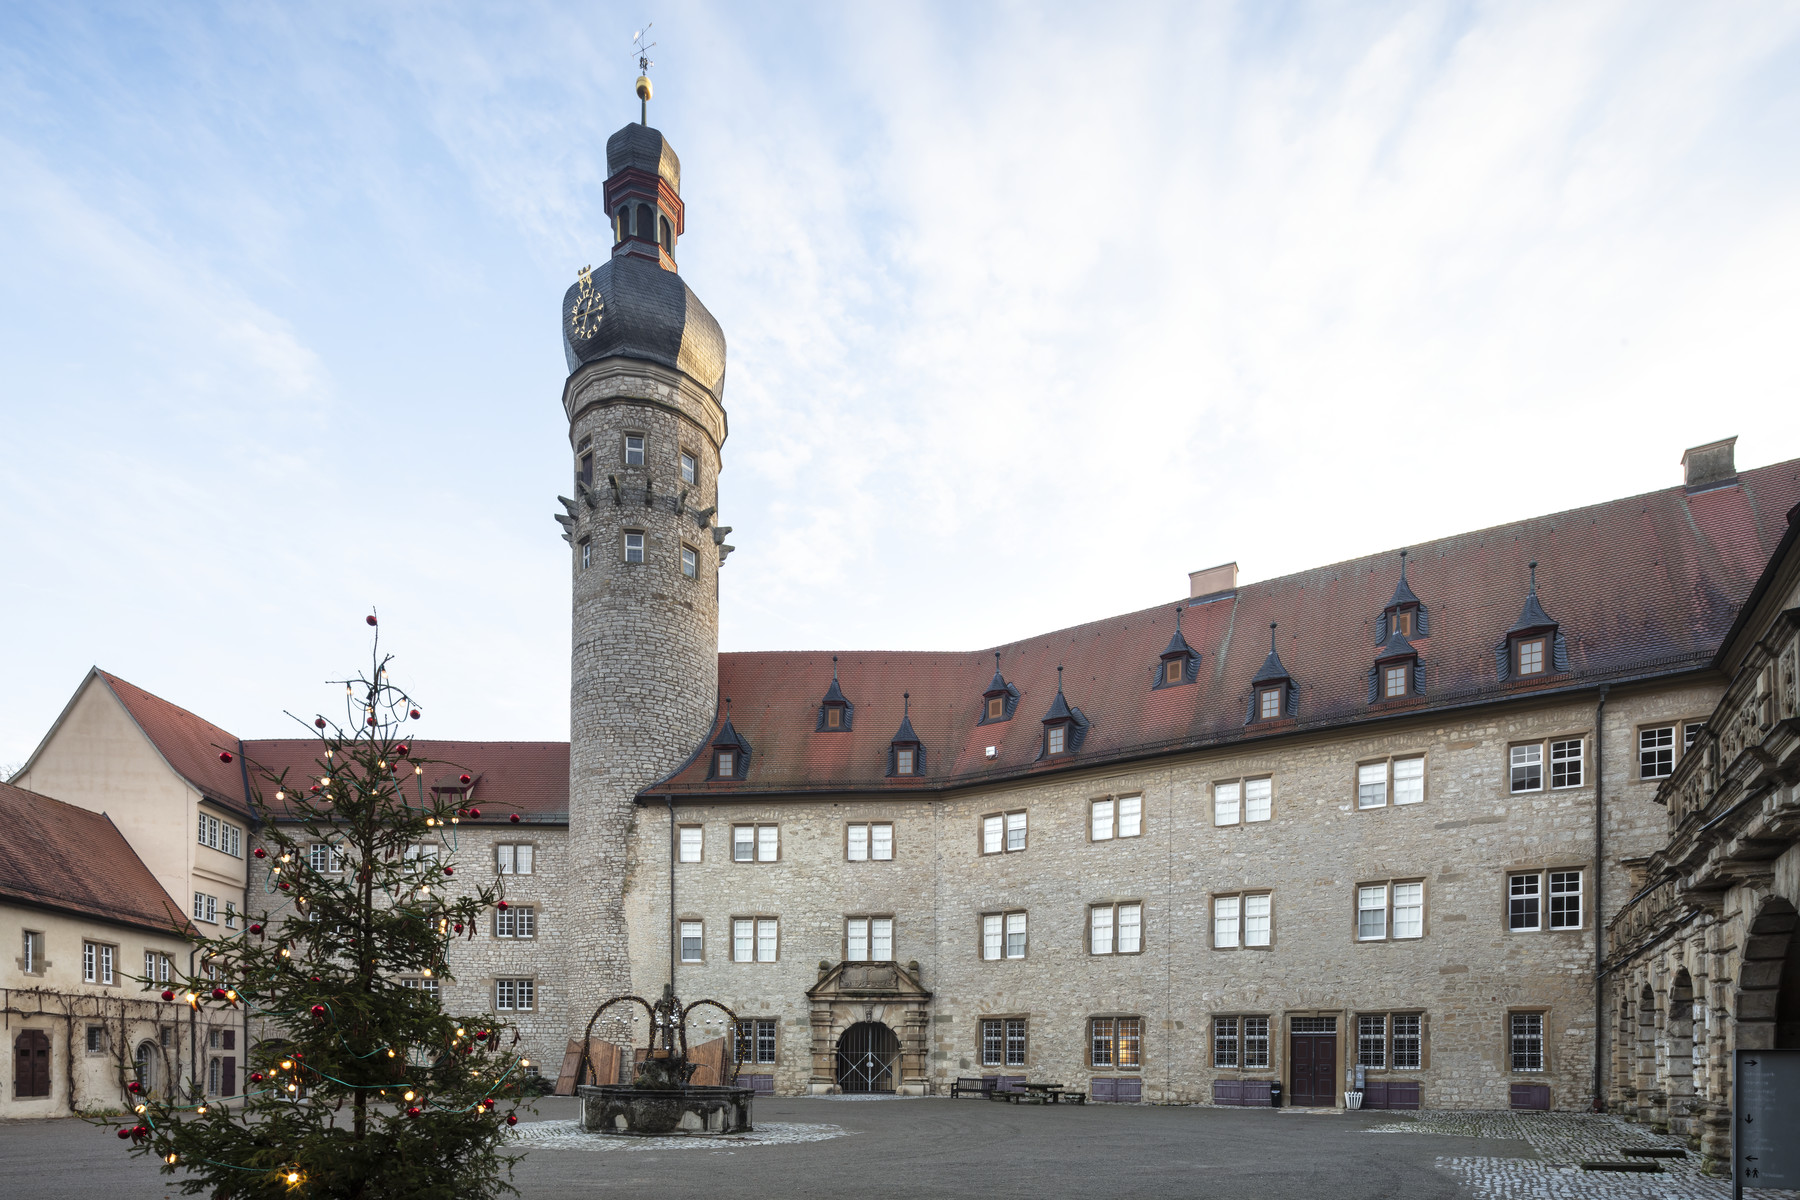
\includegraphics[height=10cm]{https://previous.bildindex.de/bilder/fmd10005902a.jpg}
  \caption{Schloss Weikersheim}
  \label{fig:{https://previous.bildindex.de/bilder/fmd10005902a.jpg}}
\end{figure}

\clearpage

\begin{figure}[H]    
  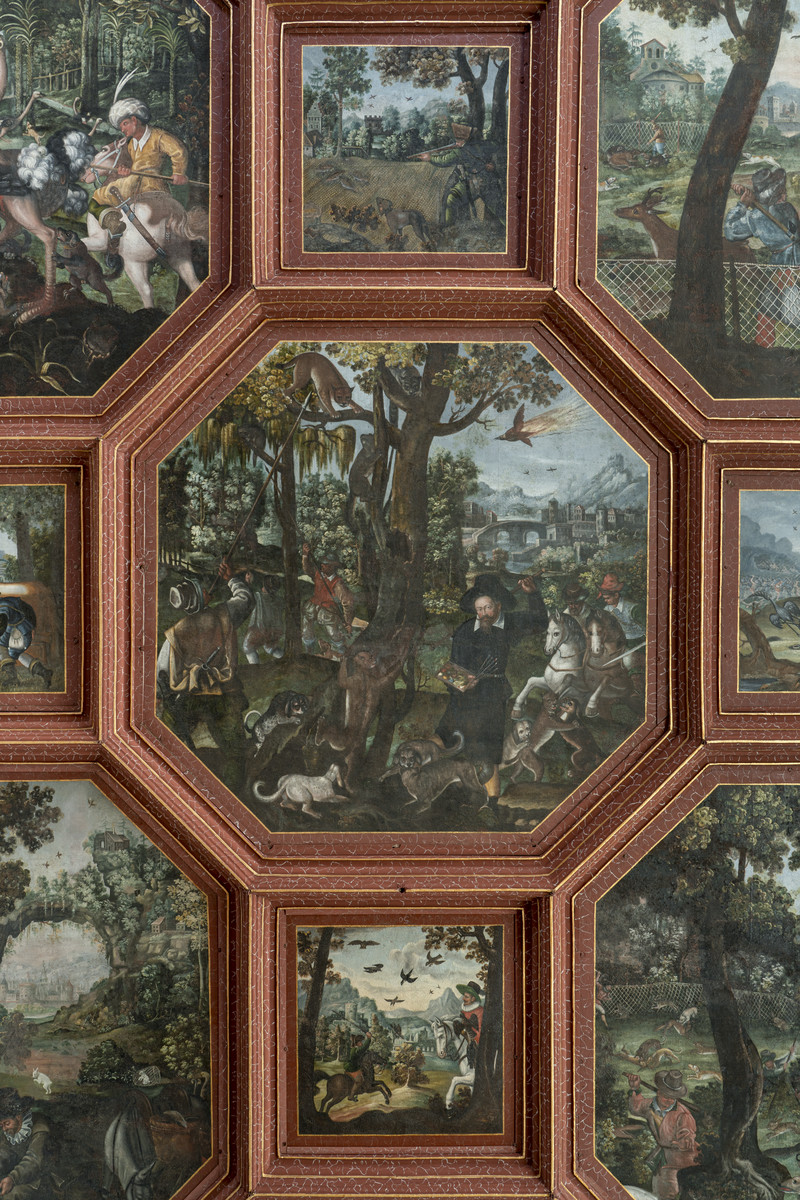
\includegraphics[height=10cm]{https://previous.bildindex.de/bilder/fmd10024325a.jpg}
  \caption{Wildkatzenjagd - General view}
  \label{fig:{https://previous.bildindex.de/bilder/fmd10024325a.jpg}}
\end{figure}

\clearpage

\begin{figure}[H]    
  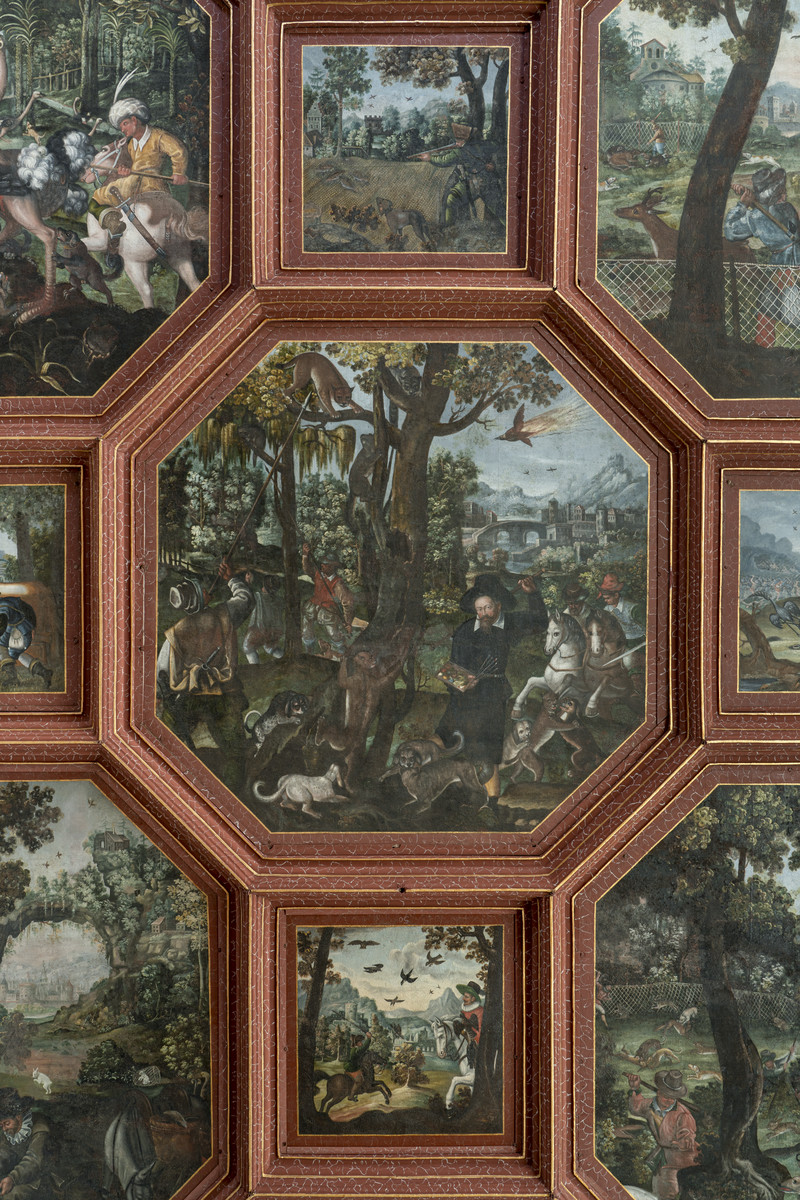
\includegraphics[height=10cm]{https://previous.bildindex.de/bilder/fmd10024325a.jpg}
  \caption{Orpheus with the Lyre and the Animals under a Tree - General View}
  \label{fig:{https://previous.bildindex.de/bilder/fmd10024325a.jpg}}
\end{figure}

\clearpage

\begin{figure}[H]    
  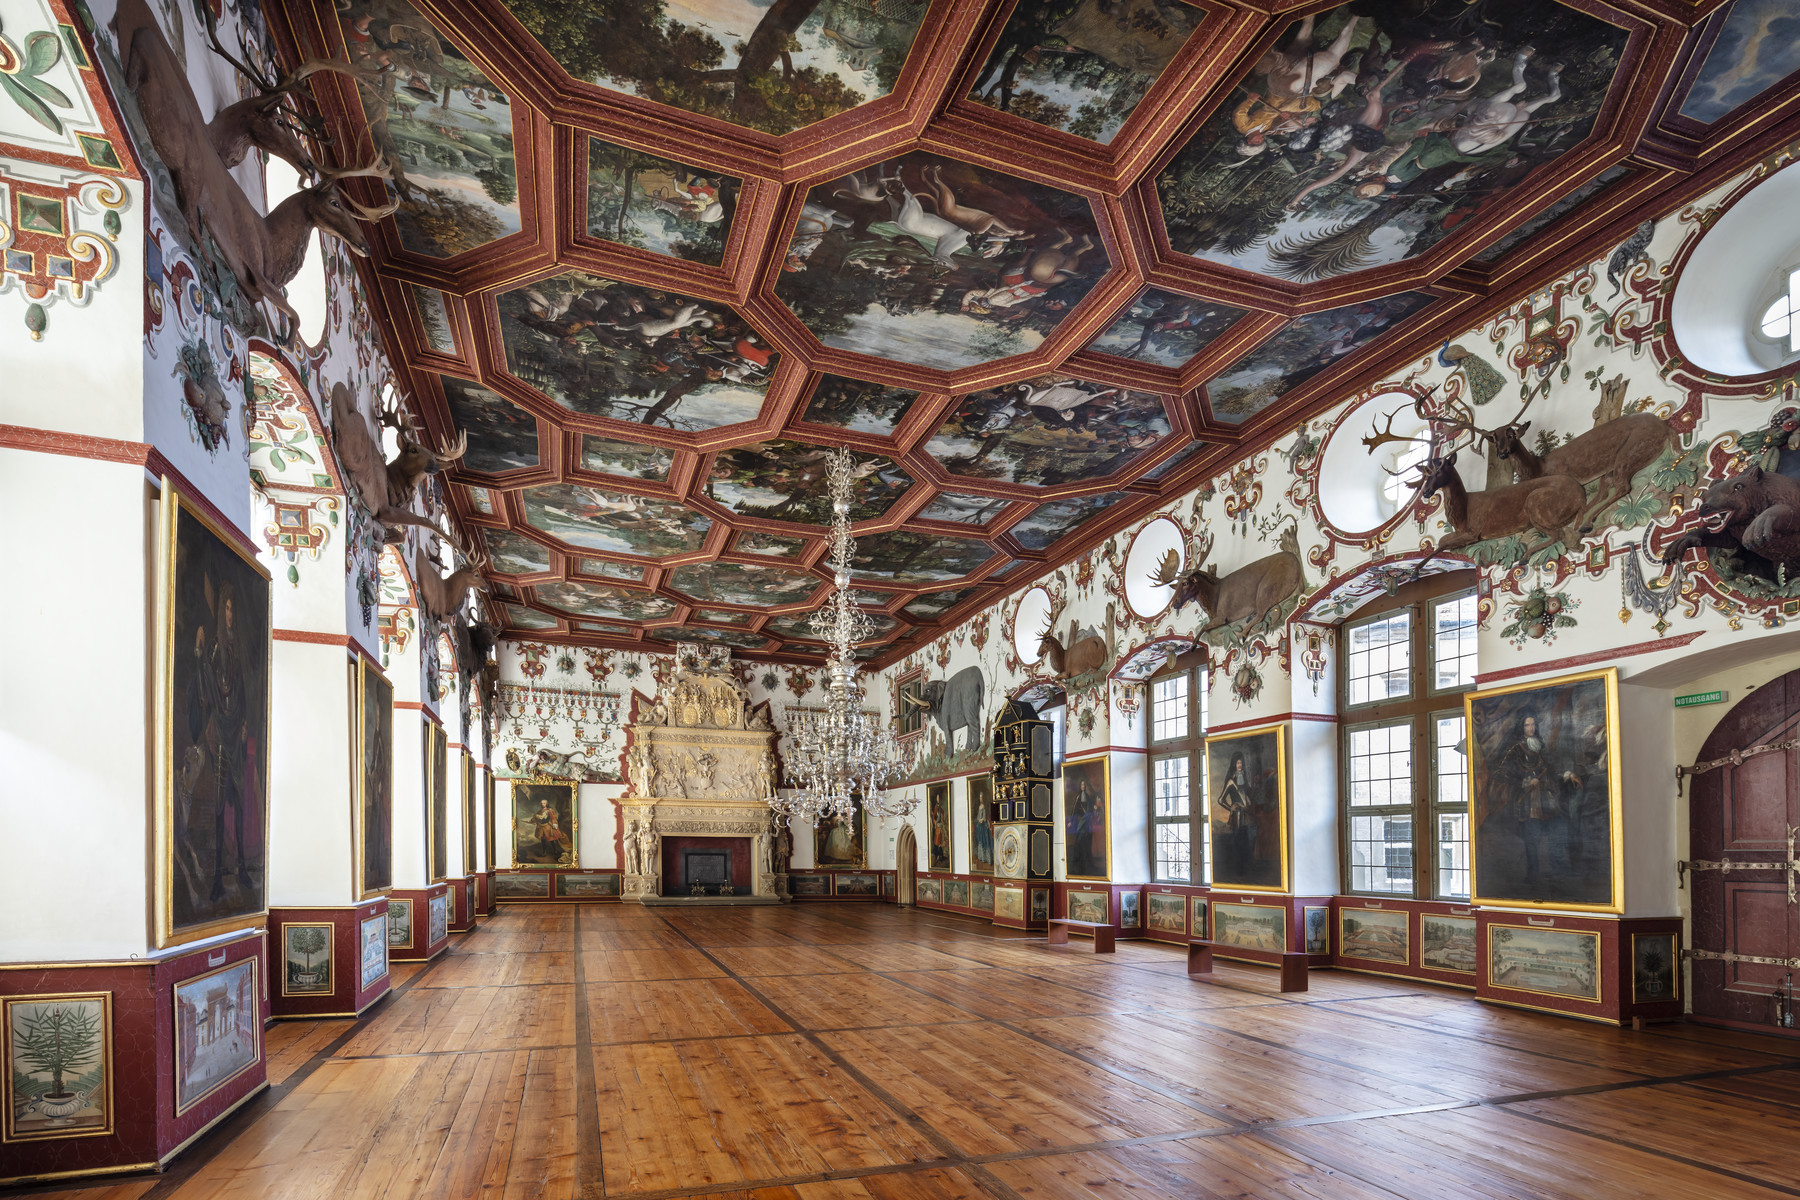
\includegraphics[height=10cm]{https://previous.bildindex.de/bilder/fmd10005859a.jpg}
  \caption{Knight's Hall + Room 72 - to the east}
  \label{fig:{https://previous.bildindex.de/bilder/fmd10005859a.jpg}}
\end{figure}

\clearpage

\begin{figure}[H]    
  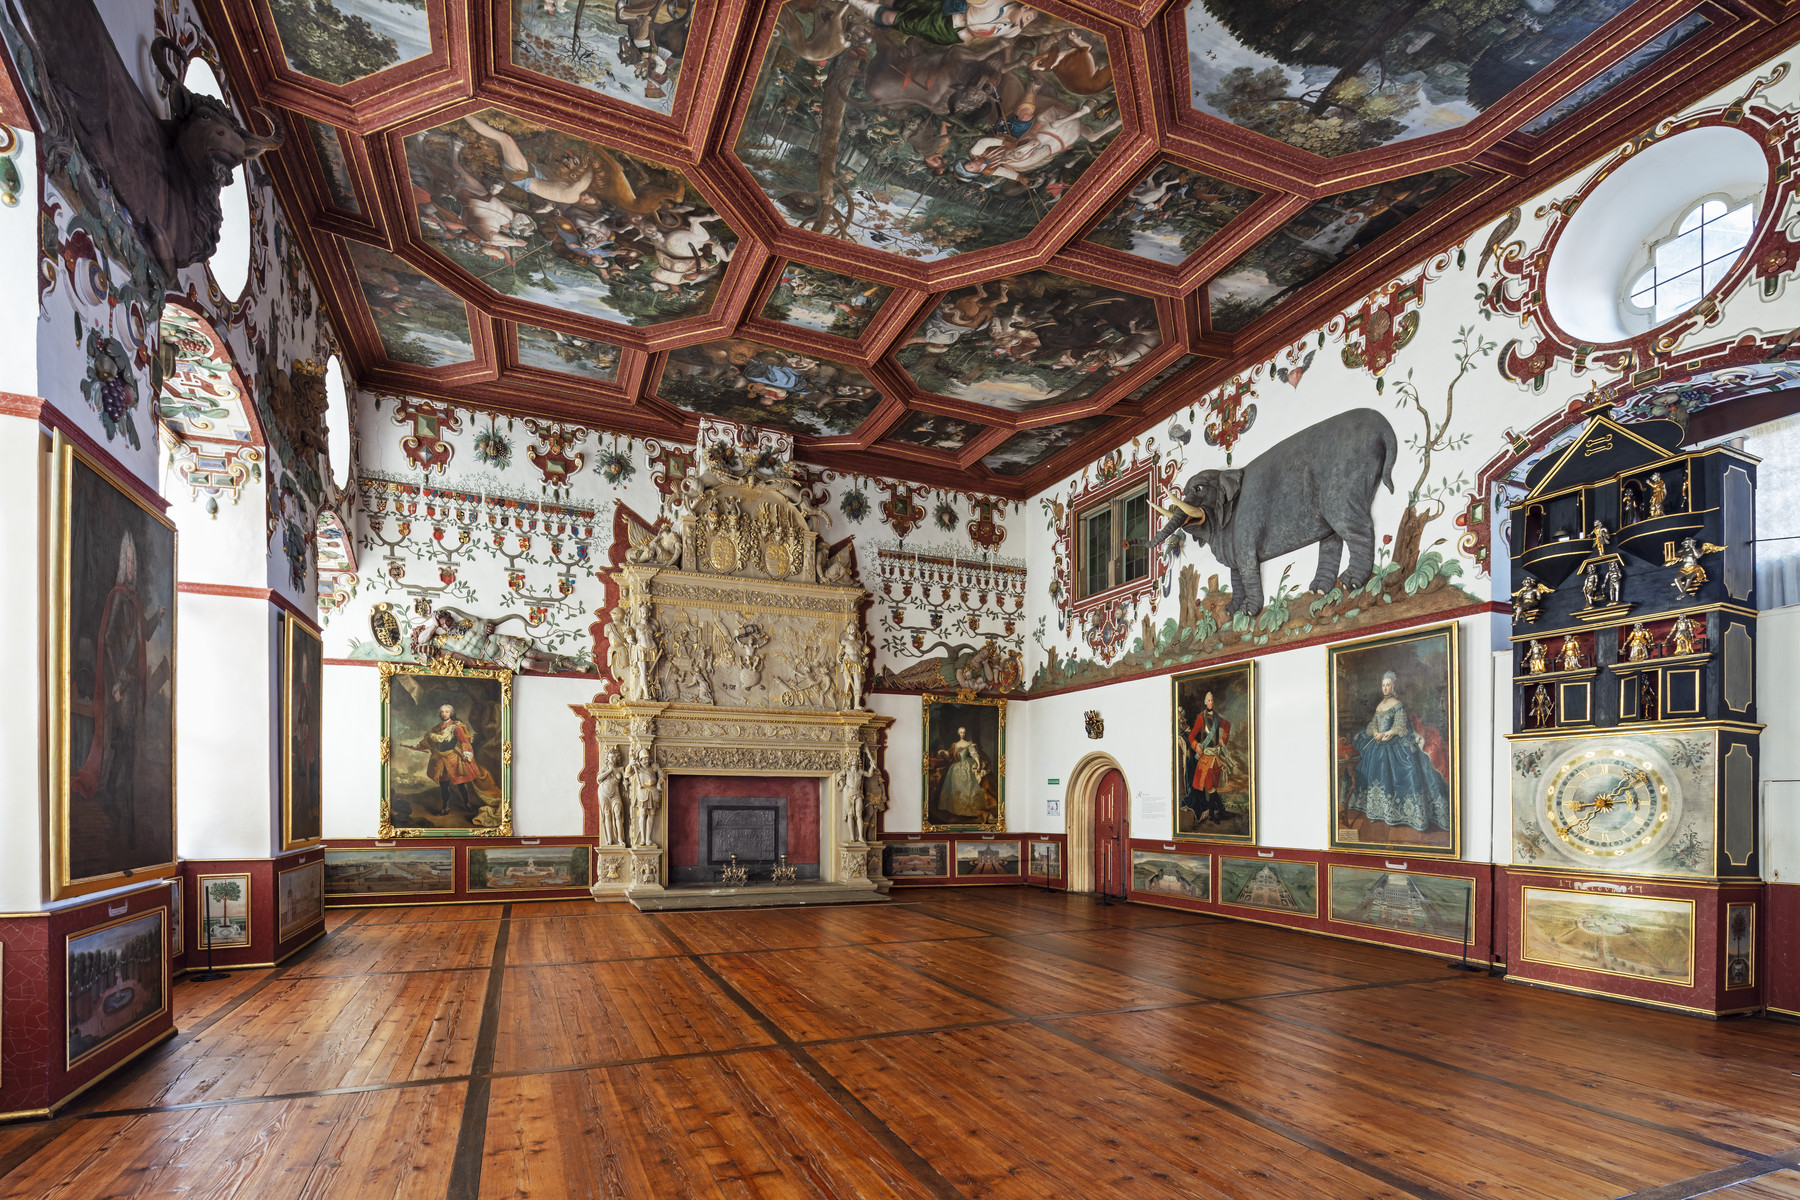
\includegraphics[height=10cm]{https://previous.bildindex.de/bilder/fmd10005860a.jpg}
  \caption{Knight's Hall + Room 72 - to the east}
  \label{fig:{https://previous.bildindex.de/bilder/fmd10005860a.jpg}}
\end{figure}

\clearpage

\end{figure*}%


\backmatter

\printindex


\end{document}
